\documentclass[parskip=full]{scrartcl}


\usepackage[T1]{fontenc}
\usepackage[ngerman,KeepShorthandsActive]{babel}
\hyphenation{TeXLa}
\usepackage[utf8]{inputenc}
\usepackage{datetime} % must be after babel
\renewcommand{\dateseparator}{-} % ISO8601 date format
\usepackage{hyperref}
\usepackage{csquotes}

\usepackage{geometry}
\usepackage[tt=false]{libertine}
\usepackage[libertine]{newtxmath}
\usepackage{microtype}
\usepackage{amsmath}
\usepackage{booktabs}
\usepackage[shortlabels]{enumitem}
\usepackage{siunitx}
\sisetup{per-mode=symbol}
\usepackage{graphicx}

\usepackage[section]{placeins}
\usepackage{xcolor}
\usepackage{tabularx}
\usepackage{longtable}

\usepackage[nameinlink]{cleveref}
\crefname{figure}{Abb}{Abb}
\setcounter{tocdepth}{2}

\usepackage{pflichtenheft}
\reversemarginpar

\widowpenalty10000
\clubpenalty10000

% ----------------------------------------------------------------------------------------------------------------------

\newcommand{\topic}{Entwicklung des graphischen Editors \texla{} zur Restrukturierung von \LaTeX"=Dokumenten}
\newcommand{\artifact}{Pflichtenheft}

\newcommand{\project}{Praxis der Softwareentwicklung}
\newcommand{\projectShort}{PSE}
\newcommand{\semester}{Sommersemester 2023}
\newcommand{\university}{Karlsruher Institut für Technologie}
\newcommand{\institute}{IPD Böhm}

\newcommand{\authors}{Paul Liebsch, Piotr Malkowski, Leonhard Mannke, Linus Schöb und Max Vogel}
\newcommand{\authorsWrapped}{Paul Liebsch, Piotr Malkowski, Leonhard Mannke, \\ Linus Schöb und Max Vogel}
\newcommand{\supervisors}{Bela Böhnke und Dennis Kobert}

\hypersetup{
  pdftitle={\projectShort: \artifact},
  bookmarks=true
}

% ----------------------------------------------------------------------------------------------------------------------

\newcommand{\zB}{z.\,B.}
\renewcommand{\dh}{d.\,h.}
\newcommand{\texla}{TeXLa}



\begin{document}

\begin{center}
\thispagestyle{empty}

  \vspace*{\fill}

  \Large
  \project \\
  im \semester

  \university, \institute

  \vspace*{5\baselineskip}

  \LARGE
  \textit{\topic}

  \textbf{\artifact}
  \Large

  \vspace*{5\baselineskip}

  \authorsWrapped

  betreut von \supervisors

  \vspace*{3\baselineskip}

  \today
  \normalsize

  \vspace*{\fill}

\end{center}

\clearpage

\tableofcontents
\clearpage

\section{Motivation}
\label{sec:motivation}

Wissenschaftliche und technische Texte werden heute oftmals in \LaTeX{} geschrieben.
Dabei gehen die Autoren meist \enquote{top-down} vor,
\dh{} man überlegt sich zunächst die Grundstruktur und Überschriften und schreibt danach den eigentlichen Inhalt.
Konsequenz dieses Vorgehens ist, dass man das Dokument später im Schreibprozess noch einmal umstrukturieren will.
In herkömmlichen Anwendungen muss man hierfür per \textit{Copy and Paste} Abschnitte des \LaTeX"=Quelltextes bewegen.
Die Vielzahl an sichtbaren Makros und Syntaxelementen stört dabei den Lesefluss.
Daher ist es leicht, die Übersicht zu verlieren oder Teile eines zu verschiebenden Abschnittes zu vergessen.

Diese Probleme geht der grafische \LaTeX"=Editor \texla{} an.
Seine intuitive Benutzeroberfläche erlaubt es, Abschnitte, Absätze, Bilder und andere Blöcke einfach per
\textit{Drag and Drop} im Dokument hin und her zu verschieben und so das Dokument zu restrukturieren.
Dabei steht die Übersicht und die Orientierung im Dokument stets an erster Stelle.

Auch bei der Erstellung der Grundstruktur kann \texla{} die Arbeit der Schreibenden vereinfachen,
da auch Überschriften erzeugt werden können und live in einer Weise dargestellt werden,
die einem Inhaltsverzeichnis ähnelt.
Insgesamt soll \texla{} also den Aufbau und die Bearbeitung gut strukturierter Dokumente unterstützen.

\clearpage
\clearpage

\section{Zielbestimmungen}
\label{sec:zielbestimmungen}
\texla{} soll es ermöglichen, \LaTeX"=Dokumente übersichtlich und hierarchisch darzustellen.
In dieser Form soll eine intuitive Benutzerschnittstelle zur Restrukturierung und Bearbeitung geboten werden.
Die Integration in bestehende Arbeitsabläufe soll über Git-Repositories und Overleaf erfolgen.

\subsection{Muss-Kriterien}
\label{subsec:muss-kriterien}
\criterium{Starten der Anwendung von der Konsole}{crt:cli}

% FA: Features der CLI: Starten, Ordner angeben, Kontrolliertes beenden
\criterium{Hierarchische grafische Darstellung von \LaTeX"=Dokumenten}{crt:hierarchy}

% FA: auch file includes unterstützen
\criterium{Erkennen von einfachen Strukturelementen}{crt:easy-elements}

% in Funktionen konkret, welche Elemente; Floats an der Stelle, an der sie im Code stehen; alle anderen als Codeblock;
% bestimmte Elemente als "bekannter Codeblock", d.h. es gibt ein Mapping von Environment auf benutzerfreundlicher Name,
% der dann als Kompaktform dienen kann (und ggf. zusätzlich angezeigt wird);
% unbekannte Inline-Makros müssen irgendwie ignoriert werden
\criterium{Erkennen von einfachen Formatierungsbefehlen}{crt:easy-format}

\criterium{Übersichtlichkeit durch automatisches Ein- und Ausblenden sowie durch Kompaktformen}{crt:clarity}

% ab durch kann man das auch in FAs auslagern
\criterium{Verschieben der Strukturelemente per Drag and Drop}{crt:dnd}

% FA: auch zwischen Ebenen
\criterium{Bearbeitung des \LaTeX"=Quelltextes von Strukturelementen mit dem Minieditor}{crt:minieditor}

\criterium{Hinzufügen von beliebigen Strukturelementen an beliebiger Stelle}{crt:add}

% Zwischenknöpfe + Minieditor, Minieditor eines anderen Elements, bekannte Strukturelemente werden erkannt und
% entsprechend angezeigt
\criterium{Persistentes Speichern von Zusatzinformationen als Kommentare in den \LaTeX"=Dateien\vspace*{-1em}}
{crt:meta-comments}

% in speziellen Kommentaren
\criterium{Benutzerdefinierter Export von \LaTeX"=Dateien}{crt:export}

% Settings panel / Profile
\clearpage

\criterium{Integration mit Git}{crt:git}

% regelmäßiges Synchronisieren, regelmäßiges Commiten nach Änderungen
\criterium{Direktlink zum entsprechenden Projekt in Overleaf}{crt:overleaf-link}

% auf konkrete Dateien geht nicht
\subsection{Kann-Kriterien}
\label{subsec:kann-kriterien}
\criteriumOptional{Konfigurierbare grafische Oberfläche}{crt:configurable-gui}

% z.B. Kommentare ausblenden
\criteriumOptional{Tastaturkürzel für häufige Operationen}{crt:keyboard}

\criteriumOptional{Hinzufügen von Notizen zu Strukturelementen}{crt:notes}

\criteriumOptional{Hinterlegen von benutzerdefinierten Kompaktformen an Strukturelementen}{crt:manual-compact-form}

\criteriumOptional{Syntax-Hervorhebung im Minieditor}{crt:syntax-highlighting}

% Minieditor?
\criteriumOptional{Code-Vervollständigung im Minieditor}{crt:code-completion}

\criteriumOptional{Möglichkeit zur einfachen Übersetzung der Anwendung}{crt:multilingual}

% FA: internationalization tool verwenden, Englisch anbieten
\criteriumOptional{Kompatibilität mit Browser-Extensions zur Autokorrektur}{crt:autocorrect}

\criteriumOptional{Automatische Zusammenfassung von Abschnitten durch KI}{crt:ai-tldrs}

% einen Knopf zur (de)aktivierung, ansonsten unsichtbar
\criteriumOptional{Unterstützung beim Schreiben durch KI}{crt:ai-rewriting}

% Vorschläge, Umschreiben nach Kommentar
\criteriumOptional{Bereitstellung als reinen Online-Dienst durch eine vorgeschaltete Login-Page}{crt:online}

\clearpage

\criteriumOptional{Feste Voreinstellungsprofile für den benutzerdefinierten Export}{crt:export-profiles}

\criteriumOptional{Export von PDF-Dateien}{crt:pdf-export}

% Voraussetzung: lokale Latex-Installation
\criteriumOptional{Verschieben von Listenelementen per Drag and Drop}{crt:lists}

\subsection{Abgrenzungskriterien}
\label{subsec:abgrenzungskriterien}
\criteriumNot{Die App ist kein vollständiger \LaTeX"=Parser oder -Compiler.}{crt:no-compiler}
Insbesondere werden keine benutzerdefinierten Makros unterstützt.

\criteriumNot{Die App muss mit fehlerhaften Dokumenten nicht umgehen können.}{crt:no-faulty-documents}
Insbesondere ist es möglich, dass der Benutzer im Minieditor invaliden oder nicht strikt hierarchischen
\LaTeX"=Quelltext (siehe~\ref{sec:produktleistungen}) schreibt und die Anwendung das resultierende Dokument nicht mehr
lesen kann.

\criteriumNot{Die App stellt keine eigene PDF-Vorschau zur Verfügung.}{crt:no-pdf-preview}

\criteriumNot{Die App stellt keine User-Verwaltung zur Verfügung, auch nicht für Git.}{crt:no-users}


\clearpage
\clearpage

\section{Produkteinsatz}
\label{sec:produkteinsatz}
Die Anwendung dient zur Restrukturierung und Bearbeitung von \LaTeX"=Dokumenten.
Sie hilft dabei, den Überblick über große Dokumente zu behalten und strukturelle Änderungen vorzunehmen,
ohne \verb|.tex|"=Dateien bearbeiten zu müssen.
Die Anwendung ermöglicht die Synchronisation mit existierenden Overleaf-Projekten.

% Import mit einfachem clone zwar auch sehr gut denkbar, aber steht erstmal in keinem Kriterium/FA
\subsection{Zielgruppe}
\label{subsec:zielgruppe}
Die Zielgruppe der Anwendung sind \LaTeX"=Benutzer.
In erster Linie sind das Wissenschaftler und andere Menschen, welche im akademischen Kontext arbeiten.
Auch Organisationen, welche technische Dokumente in \LaTeX{} erstellen, können von der Anwendung profitieren.
Die Anwendung richtet sich nicht explizit an \LaTeX"=Anfänger, da sie die Benutzung von \LaTeX{} nicht per se
vereinfacht, sondern bestimmte Abläufe effizienter und angenehmer macht.

\subsection{Betriebsbedingungen}
\label{subsec:betriebsbedingungen}
Die Anwendung folgt einem Client-Server-Modell.
Der Benutzer installiert die Server-Komponente auf seinem Computer und interagiert mit der Anwendung mittels einem
Frontend in seinem Webbrowser.
Eine Internetverbindung ist für einige Funktionen notwendig.

Eine Portierung der Server-Komponente auf einen zentral gehosteten Webserver ist möglich, jedoch nicht notwendig.


\clearpage
\clearpage

\section{Produktumgebung}
\label{sec:produktumgebung}
\subsection{Hardware}
\label{subsec:hardware}
Der Zielrechner verfügt über die folgenden oder mindestens gleichwertige Hardware-Komponenten:

\begin{itemize}
\item \textbf{CPU}: AMD Ryzen 5 5500U @4,2~\si{\giga\hertz}
  \item \textbf{RAM}: 8~\si{\giga\byte} @3.200~\si{\mega\hertz}
  \item \textbf{Speicher}: 10~\si{\giga\byte} freier Speicherplatz auf Festplatte mit 200~\si{\mega\byte\per\second}
  Übertragungsrate
  \item \textbf{Netzwerk}: Netzwerkinterface und Internetanschluss mit 50~\si{\mega\bit\per\second} Download,
  10~\si{\mega\bit\per\second} Upload
  \item \textbf{Bildschirm}: Mindestens 1920x1080~px

\end{itemize}
\subsection{Software}
\label{subsec:software}
Der Zielrechner verfügt über die folgenden Software-Komponenten:

\begin{itemize}
\item \textbf{Betriebssystem}:

\begin{itemize}
\item Windows 8 oder neuer
    \item Linux-Distribution mit Kernel @Version 4.14.x oder neuer

\end{itemize}
\item Git @Version 2.40.1
  \item TeX Live @Version 2023
  \item Webbrowser mit Support für die Standards HTML5, CSS3 und EcmaScript6

\end{itemize}

\clearpage
\clearpage

\section{Produktfunktionen}
\label{sec:produktfunktionen}

\subsection{Verpflichtende funktionale Anforderungen}
\label{subsec:verpflichtende-funktionale-anforderungen}

\texla{} soll folgende Funktionen unterstützen:

\functionality{Starten der Anwendung}{fnc:start}
\fulfills{crt:cli}

\texla{} lässt sich von der Konsole aus starten.
Dabei wird als Argument eine \LaTeX"=Datei angegeben.
\texla{} arbeitet anschließend auf dieser und den durch sie eingebundenen Dateien.

\functionality{Beenden der Anwendung}{fnc:exit}
\fulfills{crt:cli}

Über die GUI von \texla{} lässt sich das Programm kontrolliert beenden.
Dabei werden alle Änderungen lokal gespeichert und in das lokale Git-Repository sowie das Remote-Repository übernommen.

\functionality{Hierarchische Darstellung}{fnc:hierarchy}
\fulfills{crt:hierarchy}

Abschnitte in einem \LaTeX"=Dokument werden mit den Befehlen \verb|\part|, \verb|\chapter|, \verb|\section|,
\verb|\subsection|, \verb|\subsubsection|, \verb|\paragraph| und \verb|\subparagraph| auf verschiedenen Ebenen
definiert.
Basierend darauf stellt \texla{} das ausgewählte \LaTeX"=Dokument in hierarchischer Form dar.
Somit sind diese Abschnitte sogenannte Expandables.

In einer zweispaltigen Ansicht -- im Folgenden \enquote{Standardmodus} genannt -- werden dafür alle Elemente bis zu
einer gewünschten Ebene dargestellt.
Durch Auswahl eines Abschnittes bzw. durch eine entsprechende Schaltfläche in der GUI ist ein Wechsel zu einer tieferen
bzw. zu einer höheren Ebene möglich.

\functionality{Unterstützung inkludierter Dateien}{fnc:input}
\fulfills{crt:hierarchy}

In einer \LaTeX"=Datei können mittels \verb|input| weitere \LaTeX"=Dateien integriert werden.
Deren Inhalt wird ebenso in der GUI angezeigt.
Dabei entsteht für jede Verwendung von \verb|input| ein Strukturelement, dem auf tieferen Ebenen die jeweiligen
Strukturelemente der inkludierten Datei untergeordnet sind.
Somit ist \verb|input| ebenfalls ein Expandable.

\clearpage

\functionality{Strukturelemente in Blöcke aufteilen}{fnc:blocks}
\fulfills{crt:easy-elements}

Mittels \verb|\begin{...}| und \verb|\end{...}| können Umgebungen in \LaTeX"=Dokumenten genutzt werden.
\texla{} erkennt solche Umgebungen und stellt diese wie auch die genannten Abschnitte jeweils als separaten Block dar.
Umgebungen sind keine Expandables.
Ineinander verschachtelte Umgebungen werden also zu einem Block zusammengefasst und im Gegensatz zu Abschnitten nicht
auf mehrere Ebenen aufgeteilt.
Eine Ausnahme hiervon bildet die Umgebung \verb|document|.

\functionality{Bestimmte Strukturelemente rendern}{fnc:render}
\fulfills{crt:easy-elements}

Folgende Strukturelemente werden in gerenderter Form, vergleichbar mit der Ansicht im PDF-Dokument, angezeigt:

\begin{itemize}
  \item Bilder, definiert durch \verb|\includegraphics|
  \item Formeln, definiert durch \verb|\[ ... \]|, \verb|$$ ... $$| oder durch eine der Umgebungen \verb|displaymath|
  und \verb|equation|
\end{itemize}

Für alle anderen Strukturelemente reicht eine Darstellung in Form des \LaTeX"=Quelltextes innerhalb des jeweiligen
Blocks aus.

Sofern sich Elemente wie Bilder in Floats befinden, richtet sich die Position der Darstellung in \texla{} nach der
Position im Quelltext, nicht nach der Position im PDF-Dokument.

\functionality{Formatierung in Textblöcken}{fnc:format}
\fulfills{crt:easy-format}

Bei Textblöcken sowie bei Überschriften von Abschnitten werden die \LaTeX"=Befehle \verb|\textbf| und \verb|\textit|
berücksichtigt.
Entsprechende Teile des Textes werden fett bzw. kursiv hervorgehoben.

\functionality{Ein- und Ausblenden von Strukturelementen}{fnc:hide}
\fulfills{crt:clarity}

Wie in \functionalitylink{fnc:hierarchy} erläutert, stellt \texla{} nur Strukturelemente bis zur gewählten Ebene dar.
Alle Strukturelemente auf tieferen Ebenen werden ausgeblendet.
Beim Wechsel zwischen Ebenen werden automatisch die entsprechenden Elemente ein- bzw. ausgeblendet.

\clearpage

\functionality{Kompaktform von Strukturelementen}{fnc:compact}
\fulfills{crt:clarity}

Auf der linken Seite der zweispaltigen Ansicht von \texla{} werden die gleichen Expandables wie auf der rechten Seite
angezeigt.
Links werden die Elemente in kompakter Form dargestellt, rechts vollständig.

Bei Textblöcken entspricht die kompakte Darstellung den ersten Worten des Absatzes, bei Abschnitten der dazugehörigen
Überschrift, bei Bildern einer verkleinerten Anzeige des Bildes und bei sonstigen Strukturelementen dem Namen der
entsprechenden Umgebung.

Eine Ausnahme hiervon bilden Algorithmen, definiert durch eine der Umgebungen \verb|lstlisting|, \verb|minted|,
\verb|codebox| und \verb|algorithm|.
Diese werden unabhängig von der konkreten Umgebung als Algorithmus erkannt.
Die Kompaktform dieser Umgebungen entspricht dem Wort \enquote{Algorithmus} bzw. \enquote{algorithm}.

\functionality{Bereitstellung einer Graphansicht}{fnc:graph}
\fulfills{crt:hierarchy}

\texla{} bietet neben dem bisher beschriebenen Standardmodus einen \enquote{Graphmodus}, in dem alle Strukturelemente
auf allen Ebenen in Kompaktform angezeigt werden.

\functionality{Verschieben von Elementen per Drag and Drop}{fnc:drag-and-drop}
\fulfills{crt:dnd}

Im Standardmodus kann jedes Element in der rechten Spalte per Drag and Drop verschoben werden.
Der Inhalt des Strukturelements bleibt dabei unverändert.
Eine Verschiebung von der rechten in die linke Spalte ist nicht möglich.
Die von \LaTeX{} vorgegebene Grenze von maximal 7 Ebenen für Abschnitte kann beim Verschieben nicht überschritten
werden.

Im Graphmodus ist ebenso ein Verschieben beliebiger Strukturelemente an beliebige Stellen unter den bestehenden
Einschränkungen möglich.

\functionality{Bereitstellung eines Minieditors}{fnc:minieditor}
\fulfills{crt:minieditor}

Für jedes Strukturelement lässt sich im Standardmodus ein Minieditor öffnen.
Darin ist eine Bearbeitung des entsprechenden \LaTeX"=Quelltextes möglich.
Dieser Modus wird als \enquote{Bearbeitungsmodus} bezeichnet.

\clearpage

\functionality{Hinzufügen von Strukturelementen}{fnc:add}
\fulfills{crt:add}

Zwischen aufeinanderfolgenden Strukturelementen lässt sich im Standardmodus ein weiteres Strukturelement hinzufügen.
In der GUI existiert dafür eine entsprechende Schaltfläche an den jeweiligen Stellen.
Durch einen Klick darauf öffnet sich ein neuer Minieditor mit leerem Inhalt.
Der anschließend darin eingegebene \LaTeX"=Quelltext bildet das neue Strukturelement.

Alternativ lässt sich ein neues Strukturelement auch durch den jeweiligen \LaTeX"=Befehl innerhalb des Minieditors
eines bereits vorhandenen Elements erstellen.
Der ursprüngliche Block wird anschließend entsprechend in mehrere Blöcke aufgeteilt, ggf. auf verschiedenen Ebenen.

\functionality{Speichern von Zusatzinformationen in Kommentaren}{fnc:meta-comments}
\fulfills{crt:meta-comments}

Notwendige Zusatzinformationen werden innerhalb der \LaTeX"=Datei in gesonderten Kommentaren persistent gespeichert.
Diese Kommentare unterscheiden sich durch ein eindeutiges Präfix von regulären Kommentaren im \LaTeX"=Quelltext.

\functionality{Benutzerdefinierter Export}{fnc:export}
\fulfills{crt:export}

Das ausgewählte \LaTeX"=Dokument lässt sich exportieren.
Durch Einstellungsmöglichkeiten lassen sich einzelne Teile des Dokuments wie Kommentare im \LaTeX"=Quelltext vom Export
ausschließen.
Beim Export wird die ursprüngliche Ordner- und Dateistruktur beibehalten.

\functionality{Integration mit Git}{fnc:git}
\fulfills{crt:git}

\texla{} übernimmt Änderungen am \LaTeX"=Dokument stets in die entsprechenden lokalen Dateien.
Nach 5~\si{\second} ohne Änderungen erfolgt automatisch ein Commit in das lokale Git-Repository sowie ein Push in das
entsprechende Remote-Repository.

\functionality{Link zum Projekt in Overleaf}{fnc:overleaf-link}
\fulfills{crt:overleaf-link}

Die GUI bietet einen Direktlink zum entsprechenden Projekt in Overleaf, das mit dem Git-Repository verbunden ist.
Ein Direktlink zur aktuell geöffneten Datei wird nicht angeboten.

\clearpage

\subsection{Optionale funktionale Anforderungen}
\label{subsec:optionale-funktionale-anforderungen}

Zudem ergeben sich weitere optionale Funktionen für \texla:

\functionality{Konfigurierbare GUI}{fnc:configurable-gui}
\fulfills{crt:configurable-gui}

Die GUI von \texla{} lässt sich konfigurieren.
Beispielsweise lassen sich Kommentare im \LaTeX"=Quelltext ausblenden.

\functionality{Tastaturkürzel}{fnc:keyboard}
\fulfills{crt:keyboard}

\texla{} bietet Tastaturkürzel für einzelne Operationen, \zB{} das Wechseln zwischen Standardmodus und Graphmodus, an.

\functionality{Hinzufügen von Notizen}{fnc:notes}
\fulfills{crt:notes}

Zu jedem Strukturelement lässt sich über eine entsprechende Schaltfläche in der GUI eine Notiz hinzufügen.

\functionality{Benutzerdefinierte Kompaktformen von Strukturelementen}{fnc:manual-compact-form}
\fulfills{crt:manual-compact-form}

Abweichend von \functionalitylink{fnc:compact} lassen sich benutzerdefinierte Kompaktformen für Strukturelemente
festlegen.
Dafür existiert neben jedem Strukturelement eine entsprechende Schaltfläche in der GUI.

\functionality{Syntax-Hervorhebung im Minieditor}{fnc:syntax-highlighting}
\fulfills{crt:syntax-highlighting}

Im Minieditor eines Strukturelements werden \LaTeX"=Befehle farblich hervorgehoben.

\functionality{Code-Vervollständigung im Minieditor}{fnc:code-completion}
\fulfills{crt:code-completion}

Im Minieditor eines Strukturelements wird eine Code-Vervollständigung angeboten.
Beim Tippen eines \LaTeX"=Befehls werden entsprechend passende Befehle angezeigt.
Durch Auswählen eines Vorschlags wird der Befehl an der aktuellen Stelle eingefügt.

\clearpage

\functionality{Übersetzung der Anwendung}{fnc:multilingual}
\fulfills{crt:multilingual}

\texla{} bietet die Möglichkeit, weitere Sprachen für die Anwendung einzubinden.
Die Standardsprache ist Englisch.

\functionality{Kompatibilität mit Browser-Extensions zur Autokorrektur}{fnc:autocorrect}
\fulfills{crt:autocorrect}

\texla{} stellt die Kompatibilität mit einzelnen Browser-Extensions sicher, die eine Autokorrektur bezüglich
Rechtschreibung und Grammatik bieten.

\functionality{Automatische Zusammenfassung von Abschnitten durch KI}{fnc:ai-tldrs}
\fulfills{crt:ai-tldrs}

\texla{} bietet die Möglichkeit, KI-generierte Zusammenfassungen für Abschnitte als Kompaktformen zu verwenden.
Diese Funktion lässt sich durch eine entsprechende Schaltfläche in der GUI aktivieren.

\functionality{Unterstützung beim Schreiben durch KI}{fnc:ai-rewriting}
\fulfills{crt:ai-rewriting}

\texla{} bietet die Möglichkeit, Abschnitte durch KI-Unterstützung umzuschreiben.
Dazu kann ein Kommentar angegeben werden, der als Anfrage an die KI weitergegeben wird.

\functionality{Bereitstellung als reinen Online-Dienst}{fnc:online}
\fulfills{crt:online}

\texla{} wird als reiner Online-Dienst bereitgestellt, anstatt als lokale Installation verwendet zu werden.

\functionality{Voreinstellungsprofile für den benutzerdefinierten Export}{fnc:export-profiles}
\fulfills{crt:export-profiles}

Wie in \functionalitylink{fnc:export} beschrieben, bietet \texla{} beim Export noch Einstellungsmöglichkeiten.
Dafür lassen sich einzelne Profile auswählen.

\functionality{Export von PDF-Dateien}{fnc:pdf-export}
\fulfills{crt:pdf-export}

\texla{} bietet die Möglichkeit, das aktuelle Dokument als PDF-Datei zu exportieren.

\clearpage

\functionality{Verschieben von Listenelementen per Drag and Drop}{fnc:lists}
\fulfills{crt:lists}

Elemente innerhalb einer Listenumgebung wie \verb|itemize| oder \verb|enumerate| lassen sich per Drag and Drop in der
Reihenfolge umordnen.

\clearpage
\section{Produktdaten}
\label{sec:produktdaten}

Alle Daten, die persistent gespeichert werden, liegen in \LaTeX"=Quelltextdateien innerhalb des Git-Repositorys, das
die Datei umgibt, auf der \texla{} ausgeführt wurde.
Daher werden alle Benutzerdaten in diesem Repository versioniert und sowohl lokal als auch gegebenenfalls remote
gespeichert.
Diese \LaTeX"=Quelltextdateien können bereits vorher bestanden haben oder in der Anwendung erstellt worden sein.

In den \LaTeX"=Quelltextdateien werden folgende Daten gespeichert:
\begin{itemize}
  \item Gewöhnlicher \LaTeX"=Quelltext
  \item Sämtliche Zusatzinformationen von \texla{} in entsprechend gekennzeichneten Kommentaren
\end{itemize}

\clearpage
\clearpage

\section{Systemmodell}
\label{sec:systemmodell}

\paragraph{Lokalität und Git}
Zur Benutzung muss die Anwendung lokal installiert werden.
Sie wird dann auf einer Datei in einem Ordner des lokalen Dateisystems ausgeführt,
der gleichzeitig ein Git-Repository sein kann.
Das heißt, solange die Anwendung nicht läuft, sind alle persistenten Daten in den lokalen Dateien auf dem Endgerät
gespeichert.
Sie werden regelmäßig per Commit in das lokale Git-Repository und per Push auf ein ggf. vorhandenes Remote-Repository
übertragen.

\paragraph{Overleaf}
Gegebenenfalls werden Links zu Overleaf angeboten --
diese dienen jedoch nur der Weiterleitung des Users und nicht zur Kommunikation zwischen den beiden Diensten.

\paragraph{Backend}
Für das Backend inklusive \textit{CLI} wird die Programmiersprache Rust verwendet.
Für den automatischen Import werden ein \textit{Directory Watcher} und Git verwendet.
Für das Parsen von und Arbeiten auf \LaTeX"=Dokumenten wird ein \textit{abstrakter Syntaxbaum} (\textit{AST})
verwendet.
Dieser AST stellt zu jeder Zeit den aktuell gültigen Stand der Dinge dar.

\paragraph{Frontend}
Das Frontend ist eine Web-Applikation, die im Browser ausgeführt und angezeigt wird.
Für das Frontend werden TypeScript und das Web-Framework \textit{Svelte} verwendet.
Das Rendering des \LaTeX"=Quelltextes im AST geschieht im Frontend.

\paragraph{Kommunikation}
Für die Kommunikation zwischen Backend und Frontend werden eine \textit{REST-API} und das JSON-Dateiformat
verwendet.
Insbesondere verschickt das Frontend an das Backend Befehle zur Manipulation des AST und
das Backend bietet eine Schnittstelle zum Lesen des aktuellen AST.

\clearpage
\section{Produktleistungen}
\label{sec:produktleistungen}

\texla{} garantiert unter den folgenden Voraussetzungen, die aufgeführten Anforderungen zu erfüllen:

\begin{itemize}
  \item Die zu bearbeitenden \verb|.tex|"=Dateien befinden sich lokal auf dem Zielrechner in einem Git-Repository,
  das mit einem Remote-Repository verknüpft ist.
  \item Die Dateigrößen aller zu bearbeitenden \verb|.tex|"=Dateien überschreiten in der Summe nicht
  100~\si{\kilo\byte}.
  \item Die zu bearbeitenden \verb|.tex|"=Dateien sind \textbf{strikt hierarchisch} aufgebaut.
  \item Die zu bearbeitenden \verb|.tex|"=Dateien verfügen über höchstens 5 Ebenen der hierarchischen Verschachtelung.
  \item Abschnitte werden in den zu bearbeitenden \verb|.tex|"=Dateien nicht innerhalb von \LaTeX"=Umgebungen
  geöffnet.
  Die einzige Ausnahme ist die Umgebung \verb|document|.
\end{itemize}

\textbf{Strikt hierarchisch} beschreibt ein \LaTeX"=Dokument, für das Folgendes gilt:

\begin{itemize}
  \item Jeder Abschnitt, der geöffnet wird, wird innerhalb des ihm übergeordneten Abschnitts geöffnet.
  Die höchste Abschnittsebene des Dokuments ist hiervon ausgenommen.
  Folgende Abschnittsebenen werden unterstützt:
  \verb|part|, \verb|chapter|, \verb|section|, \verb|subsection|, \verb|subsubsection|, \verb|paragraph| und
  \verb|subparagraph|.

  \textbf{Beispiel:}
  \begin{verbatim}
\section{Heading1}
\subsection{Subheading1}
  \end{verbatim}

  \textbf{Gegenbeispiel:}
  \begin{verbatim}
\section{Heading1}
\subsubsection{Subsubheading1}
  \end{verbatim}

  \clearpage

  \item \verb|input| kann auf jeder Ebene geöffnet werden.
  Für jeden Abschnitt und \verb|input| ist entweder der komplette Abschnitt innerhalb des \verb|input| oder der
  komplette \verb|input| innerhalb des Abschnitts.

  \textbf{Beispiel:}
  \begin{verbatim}
\section{Heading1}
/input{file1}
\section{Heading3}

file1.tex:
\section{Heading2}
  \end{verbatim}

  \textbf{Gegenbeispiel 1:}
  \begin{verbatim}
\section{Heading1}
/input{file1}
Some text

file1.tex:
\section{Heading2}
  \end{verbatim}

  \textbf{Gegenbeispiel 2:}
  \begin{verbatim}
\section{Heading1}
/input{file1}
\section{Heading3}

file1.tex:
Some text
\section{Heading2}
  \end{verbatim}
\end{itemize}

\clearpage
\section{GUI-Entwürfe}
\label{sec:gui-entwuerfe}

\subsection{Sidebar}
\label{subsec:sidebar}

Die Sidebar beinhaltet von oben nach unten das Logo, einen Button zum Speichern, einen Button zu Overleaf, einen Button
zum Exportieren, eine Statusanzeige, einen Graphmodus-Toggle und einen Button zum Schließen.

\subsubsection{Export}

Nachdem der Export-Button gedrückt wurde, erscheint ein Popup-Fenster.

\begin{center}
  \begin{minipage}{0.5\linewidth}
    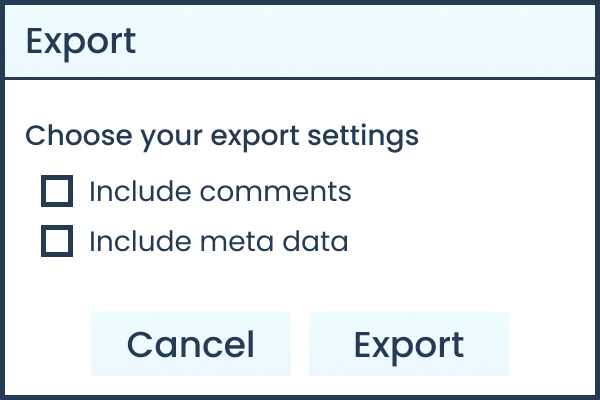
\includegraphics[width=\textwidth]{assets/img/Export_Box}
    \captionof{figure}{Export-Box mit Export"=Attributauswahl}
  \end{minipage}
\end{center}

Im Export-Fenster kann der User Exporteinstellungen wählen und den Export bestätigen oder abbrechen.

\subsubsection{Overleaf-Link}

Durch Klicken des Overleaf-Symbols gelangt man zur verknüpften Overleaf-Projektseite.

\subsubsection{Graphmodus-Toggle}

Der Button wechselt zwischen dem Graphmodus und dem Standardmodus.

\subsection{Arbeitsbereich}
\label{subsec:arbeitsbereich}

Der Arbeitsbereich, also der Bereich, der nicht Sidebar ist, besitzt drei verschiedene Modi.

\subsubsection{Standardmodus}

\begin{minipage}{\linewidth}
  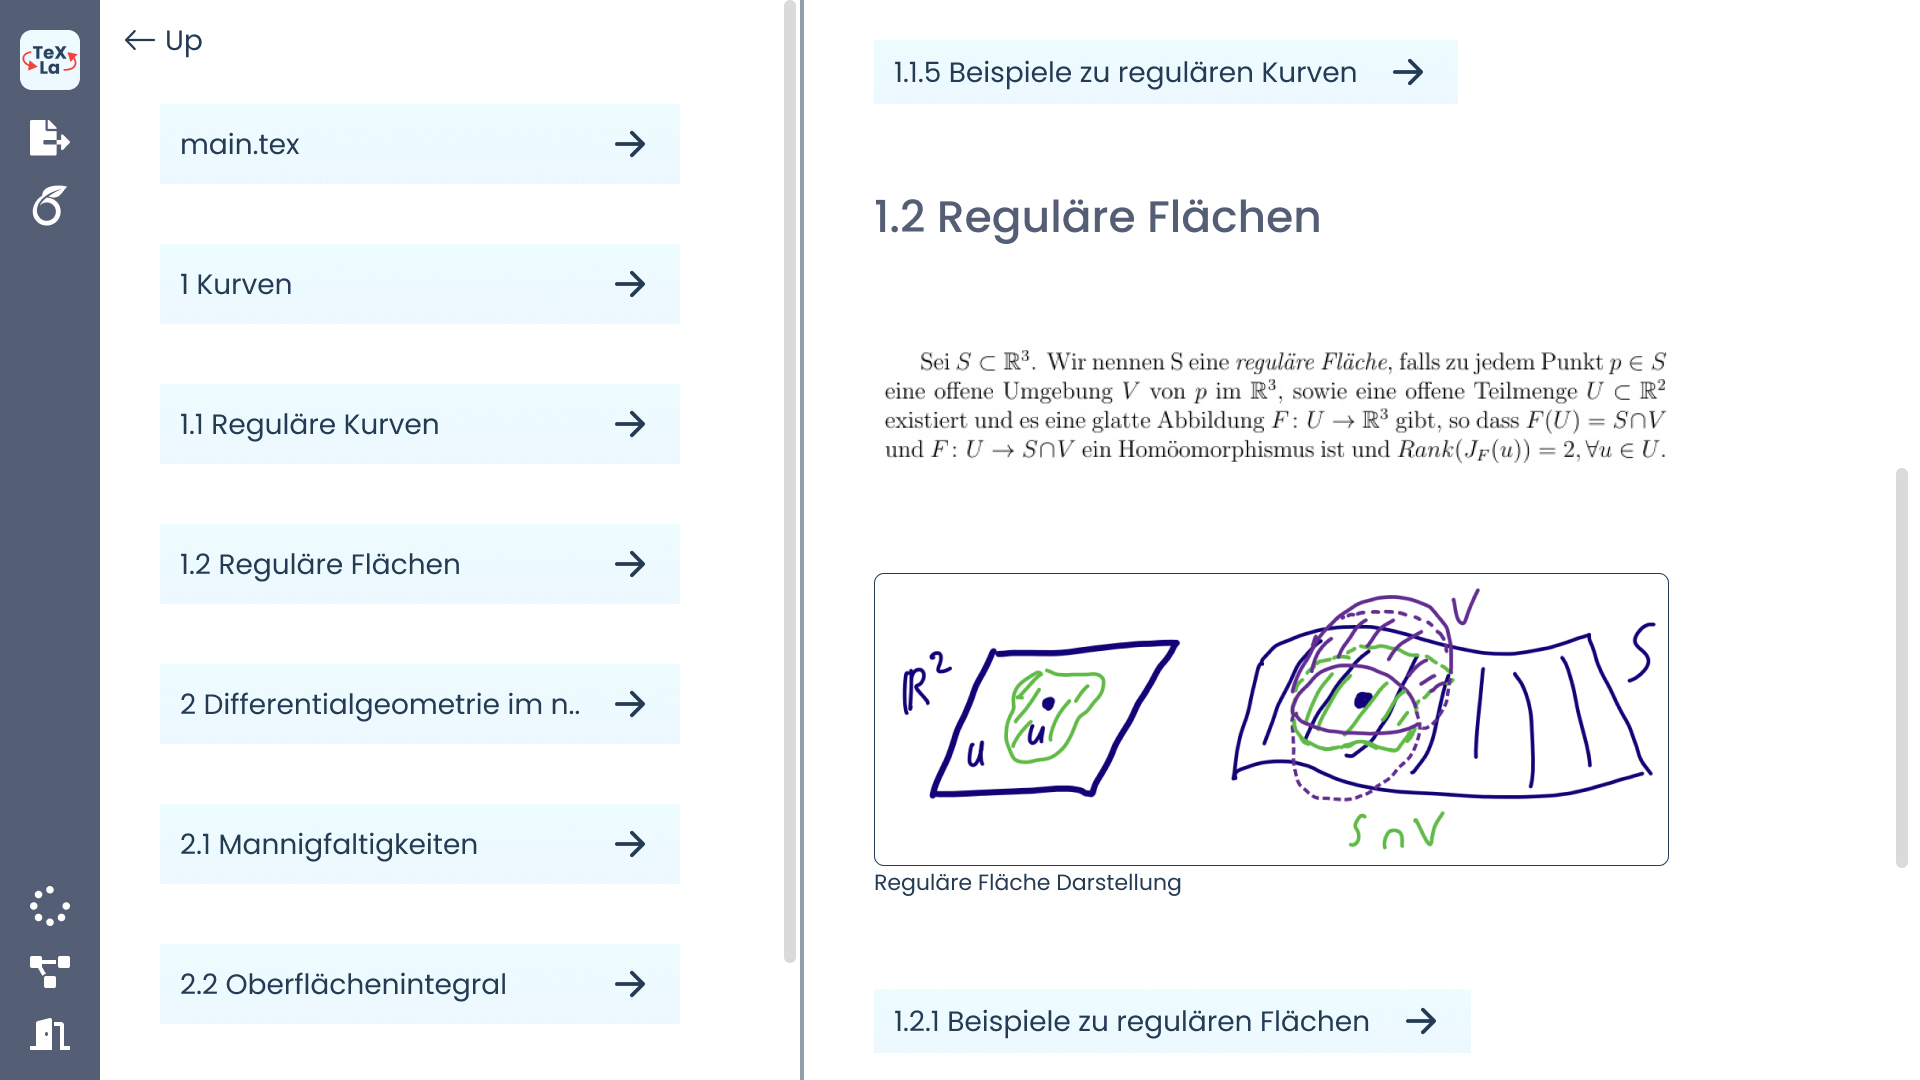
\includegraphics[width=\textwidth]{assets/img/Standardansicht}
  \captionof{figure}{Standardmodus}
\end{minipage}

In diesem Modus stehen die meisten Funktionen von \texla{} zur Verfügung.

Die rechte Spalte beinhaltet alle Strukturelemente bis Ebene $i$.
Dabei werden Expandables der Ebene $i$ in Kompaktform dargestellt und alle anderen Elemente in vollständiger Form.
In der linken Spalte werden alle Expandables des Dokuments bis zur Ebene $i-1$ in ihren Kompaktformen in
Reihenfolge des Vorkommens im Dokument dargestellt.

Auf beiden Seiten kann gescrollt werden, um den gesamten Inhalt einzusehen.
Ein Klick auf eine Kompaktform auf der linken Seite führt zu einem Sprung an die jeweilige Stelle auf der rechten Seite.

\subsubsection{Bearbeitungsmodus}

\begin{minipage}{\linewidth}
  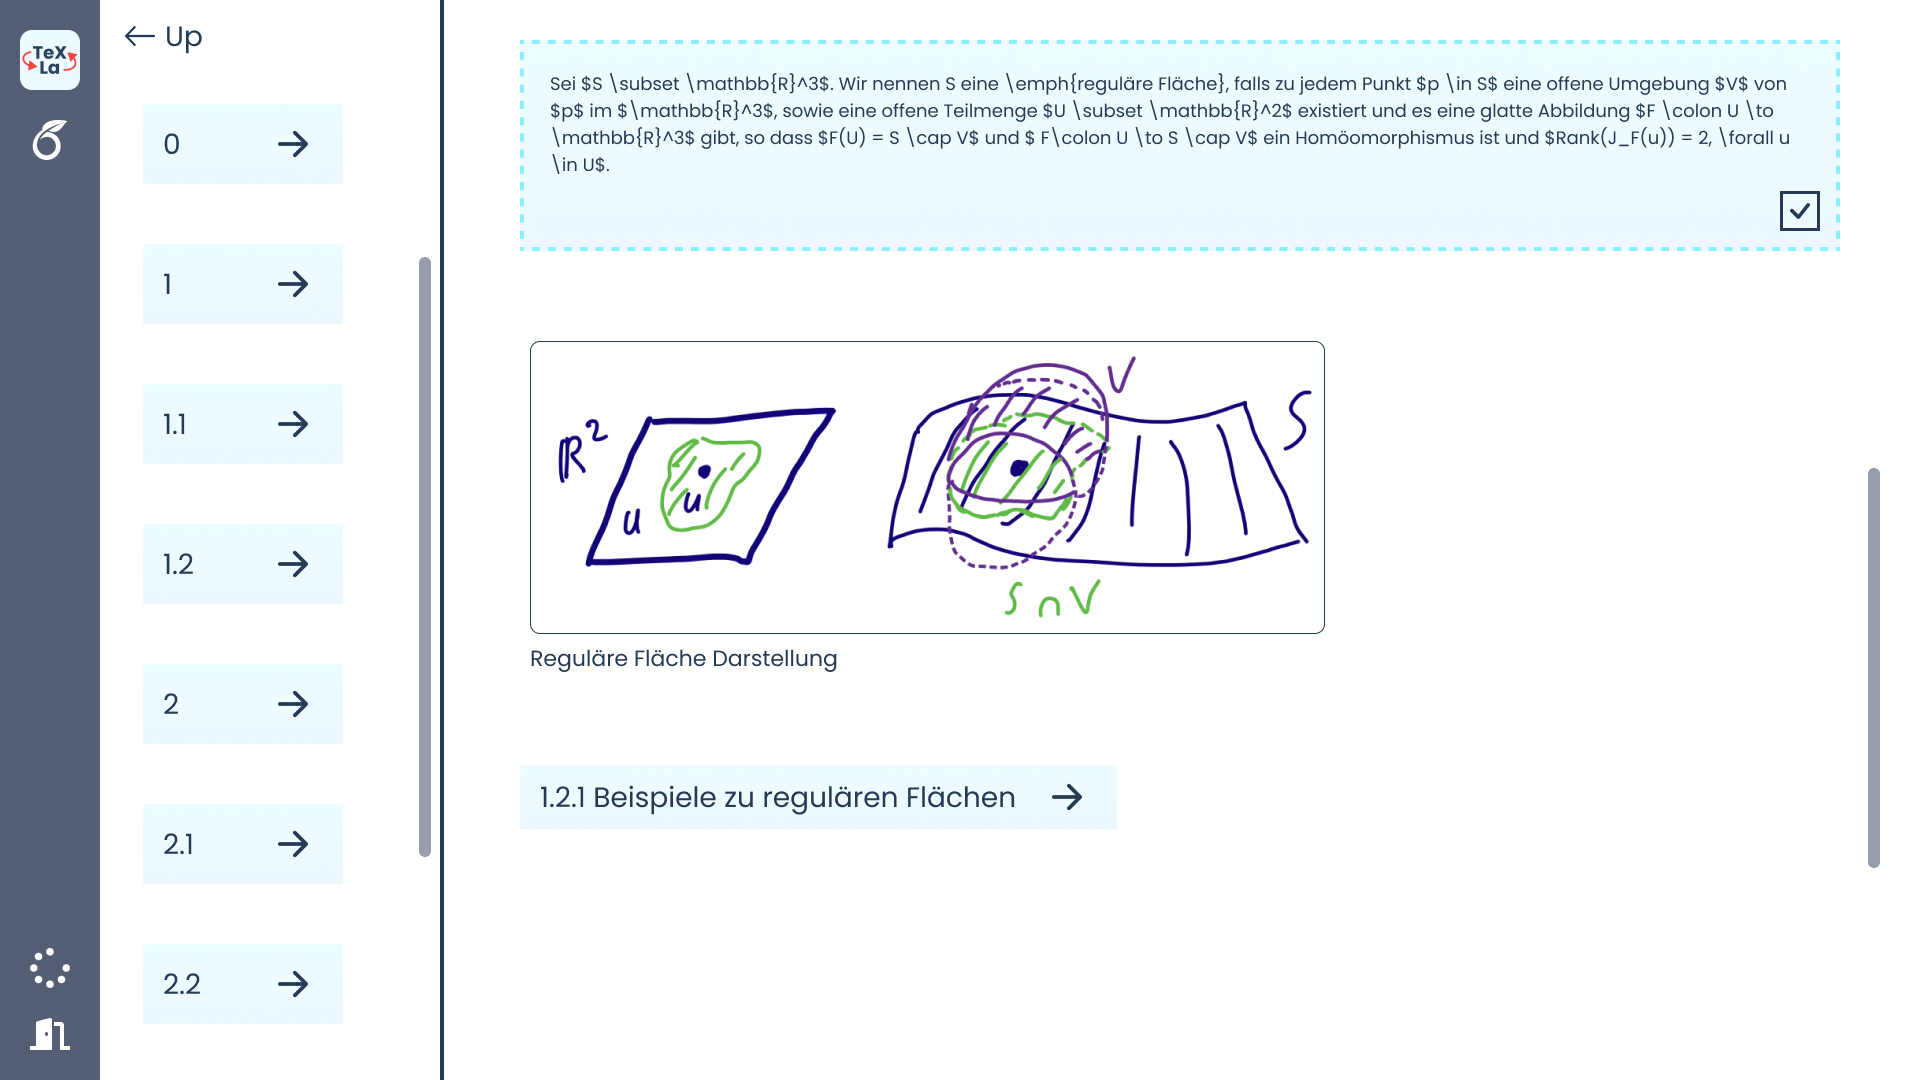
\includegraphics[width=\textwidth]{assets/img/Editor_View}
  \captionof{figure}{Bearbeitungsmodus}
\end{minipage}

Beim Bearbeiten eines Elements wechselt der Navigationsbereich in den Bearbeitungsmodus.
Hier wird die linke Spalte nur noch komprimiert dargestellt und die rechte Spalte vergrößert sich.
Das zu bearbeitende Element wird im Minieditor in Quelltext angezeigt.
Der User kann die nötigen Bearbeitungsschritte tätigen.
Durch Klicken des Bestätigen-Buttons werden die Änderungen übernommen, der User verlässt den Bearbeitungsmodus und
gelangt in den Standardmodus zurück.

\subsubsection{Graphmodus}

\begin{minipage}{\linewidth}
  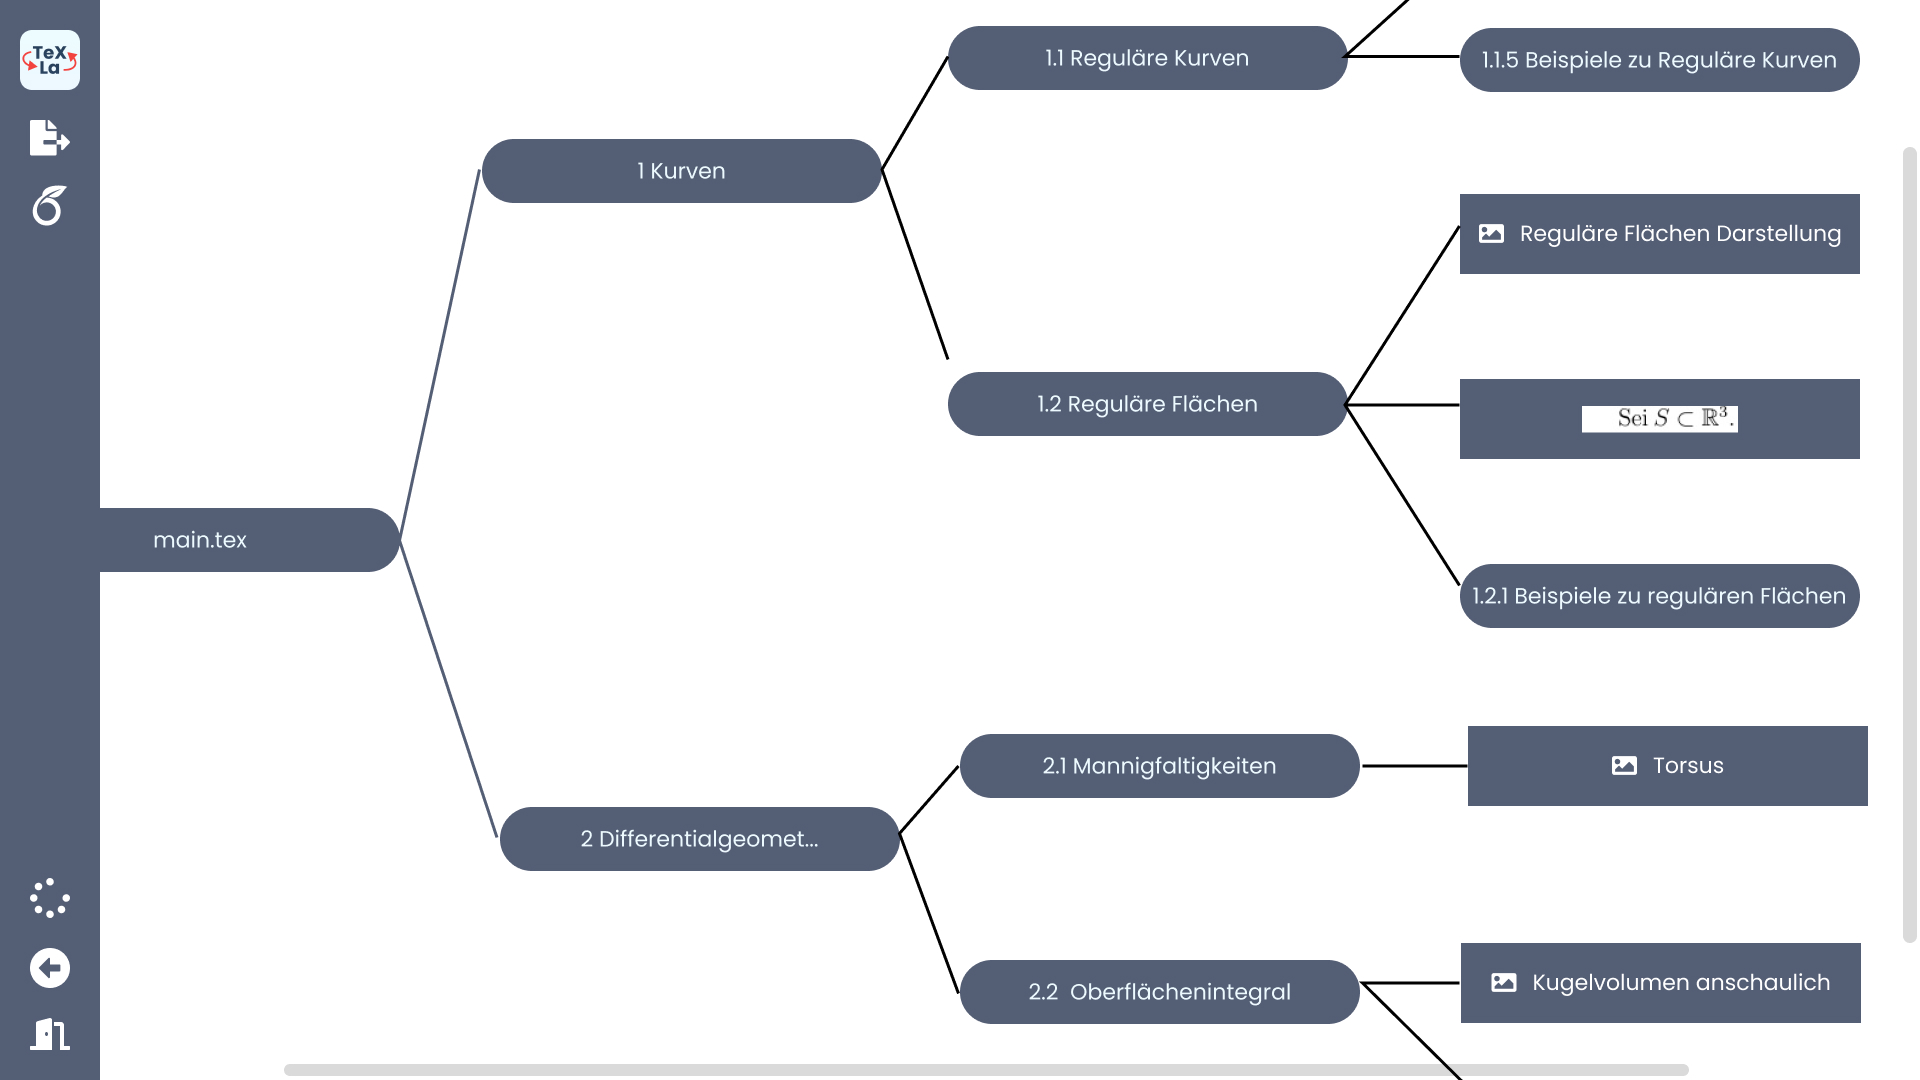
\includegraphics[width=\textwidth]{assets/img/Graphansicht}
  \captionof{figure}{Graphmodus}
\end{minipage}

Im Graphmodus wird das Dokument als Graph dargestellt.
In diesem Modus erhält der User Überblick über das Dokument und er kann die Elemente des Dokuments ebenenübergreifend
restrukturieren.
Im Graphmodus navigiert man durch Scrollen.

\subsection{Interaktion mit Elementen}
\label{subsec:interaktion-mit-elementen}

\subsubsection{Element fokussieren}

\begin{minipage}{\linewidth}
  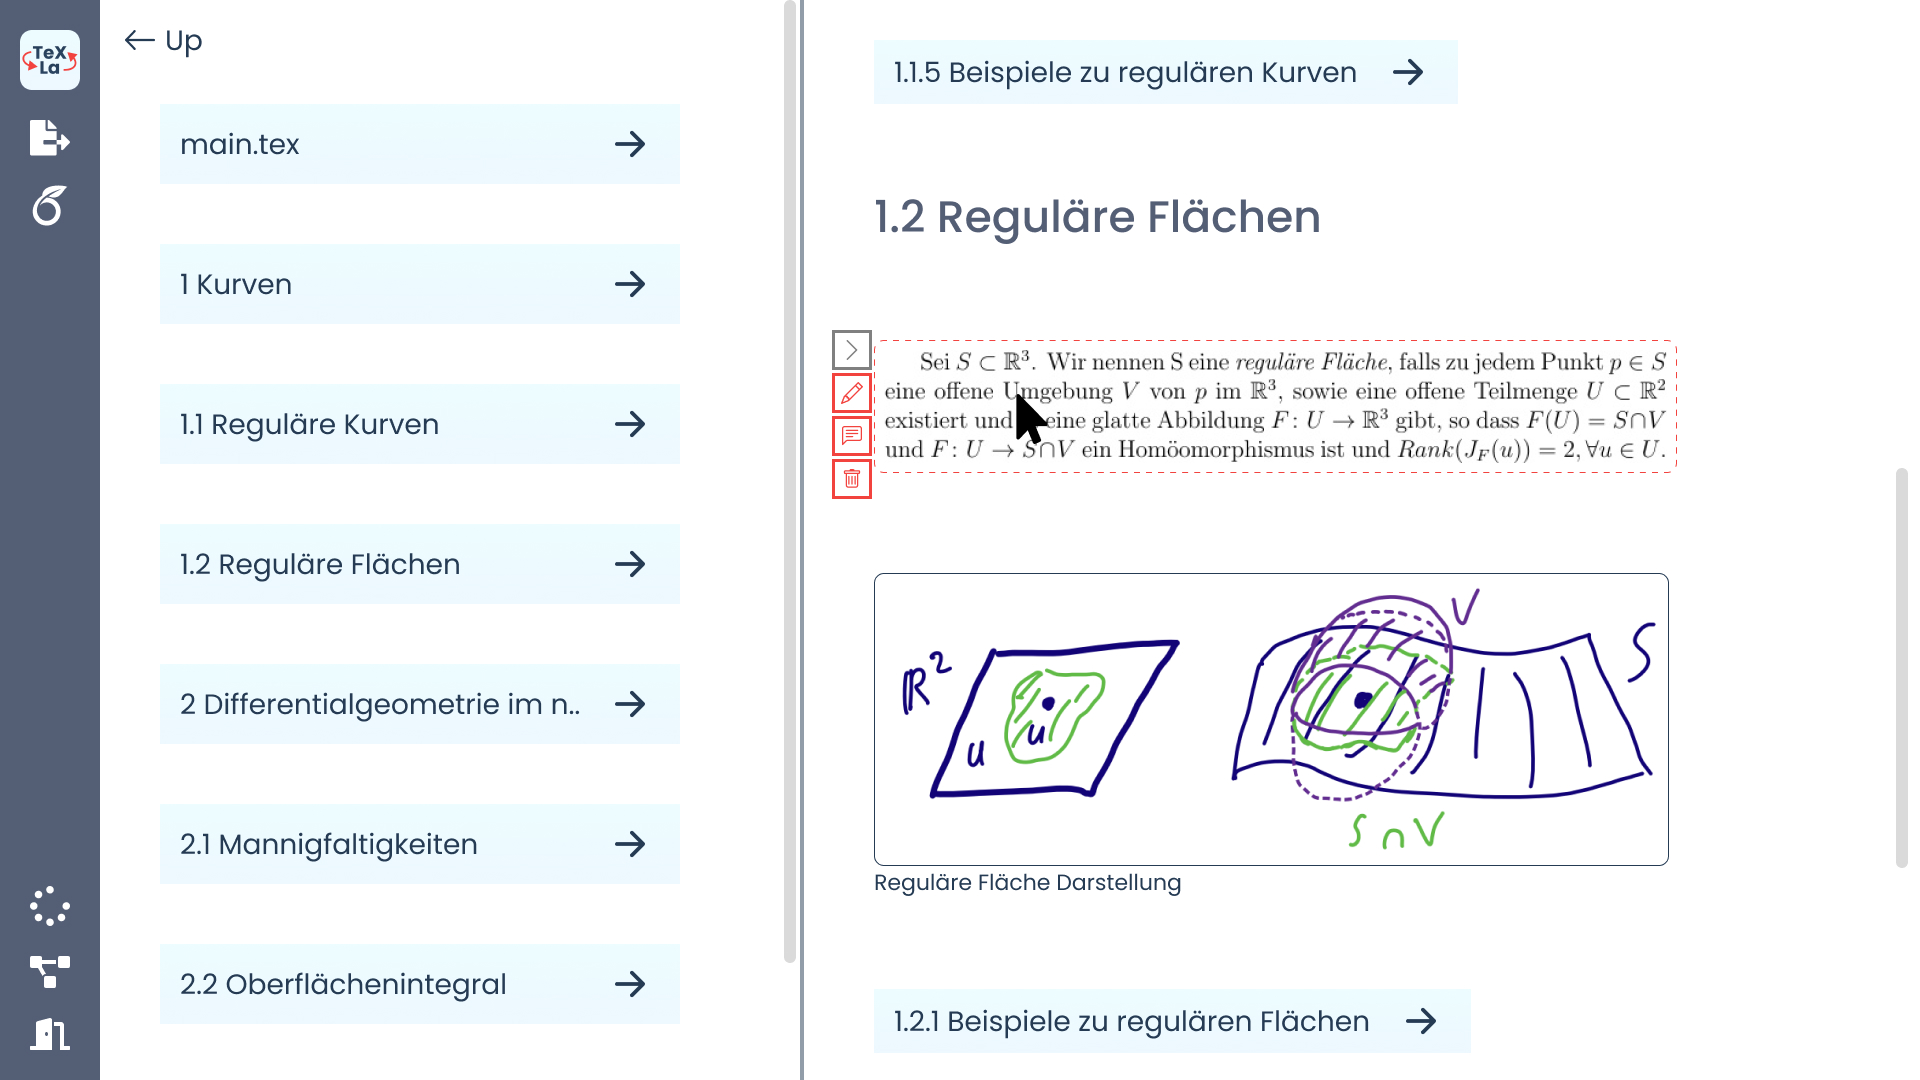
\includegraphics[width=\textwidth]{assets/img/Item_Selected_Hover}
  \captionof{figure}{Element fokussieren}
\end{minipage}

Ein Element in der Standardansicht kann in der rechten Spalte durch Hovern fokussiert werden.
Es erscheint eine Seitenleiste mit den Optionen \enquote{Expandable auswählen}, \enquote{Bearbeiten} und
\enquote{Löschen}.
Die erste Option ist nur bei Expandables aktiv und nutzbar.

\subsubsection{Löschen}

Diese Option löscht das fokussierte Element.

\subsubsection{Expandable auswählen}

\begin{minipage}{\linewidth}
  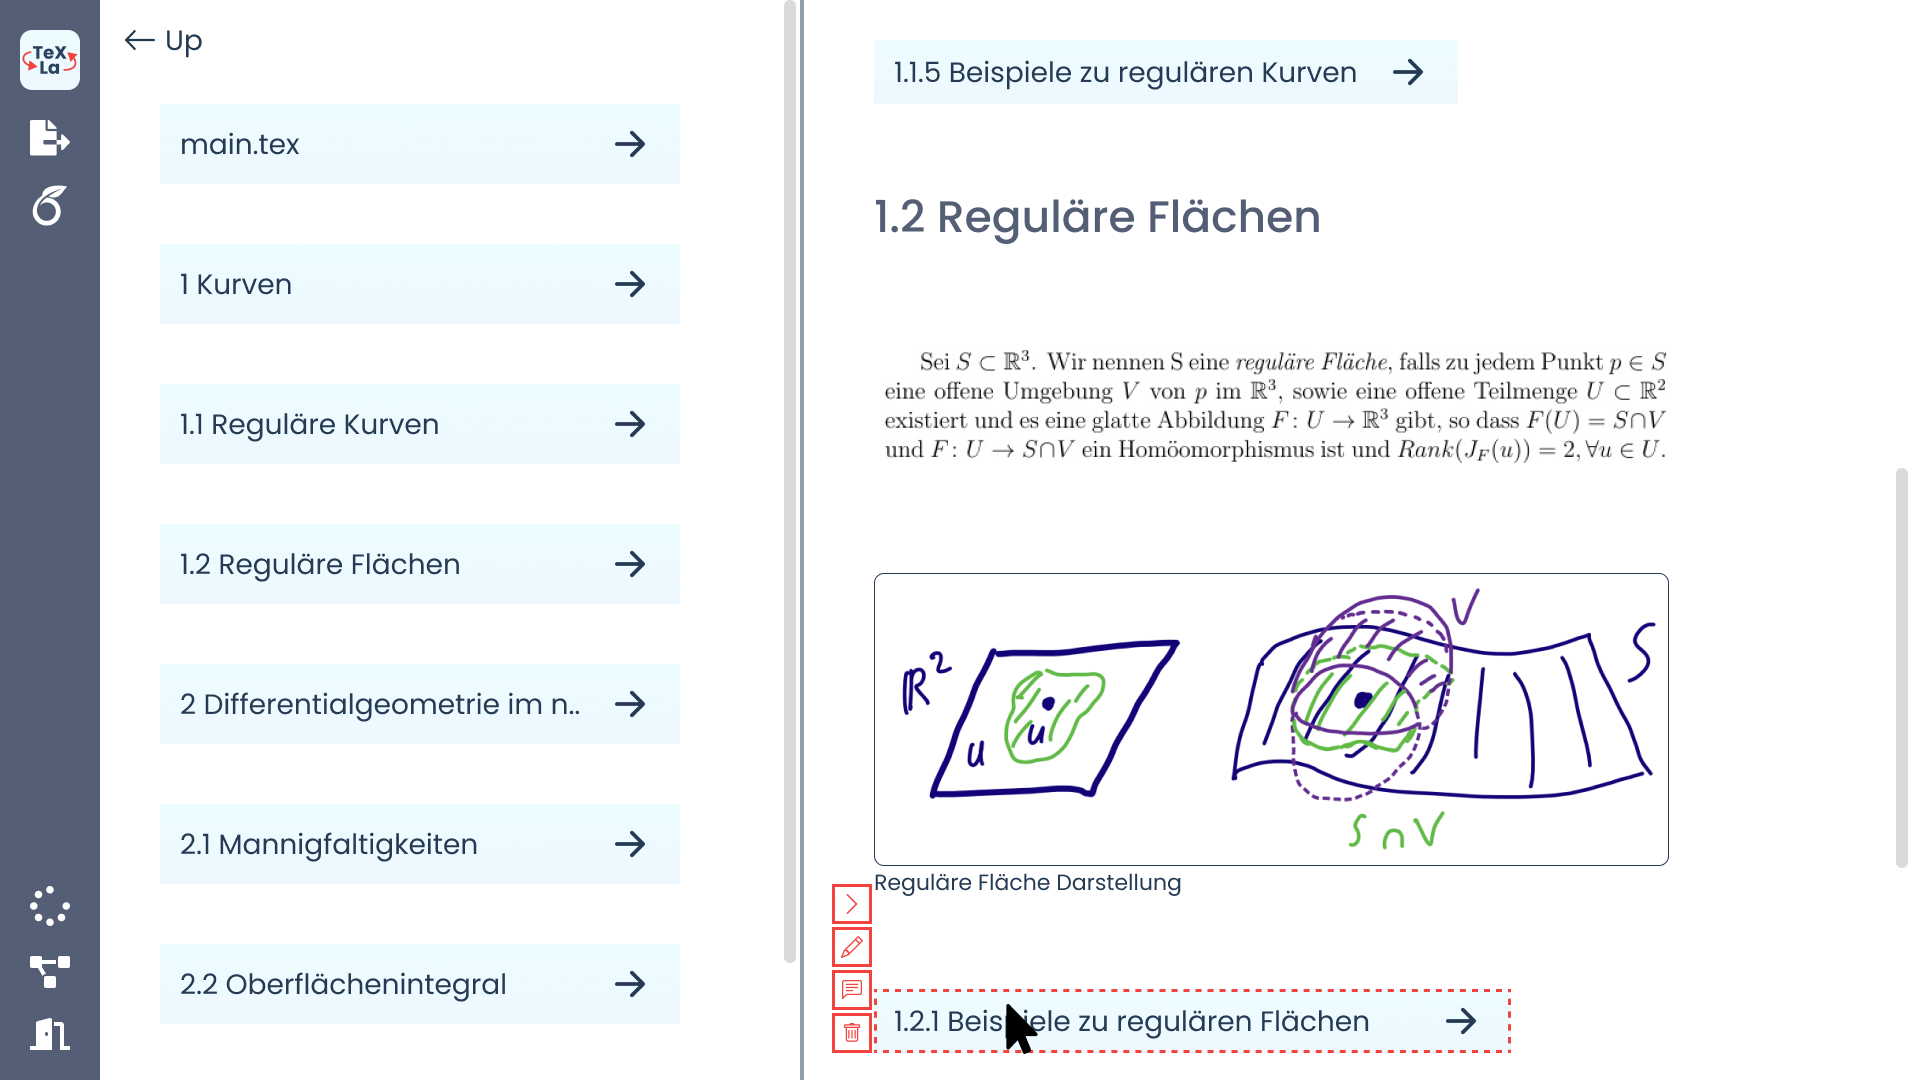
\includegraphics[width=\textwidth]{assets/img/Select_Expandable}
  \captionof{figure}{Expandable auswählen}
\end{minipage}

Durch Klicken der \enquote{Expandable auswählen}-Option bei fokussierten Expandables in der rechten Spalte wechseln
beide Spalten eine Ebene niedriger.
Durch einen Klick auf den Up-Button links oben im Navigationsbereich wechseln beide Spalten eine Ebene höher.

\subsection{Element hinzufügen}
\label{subsec:element-hinzufuegen}

\begin{minipage}{\linewidth}
  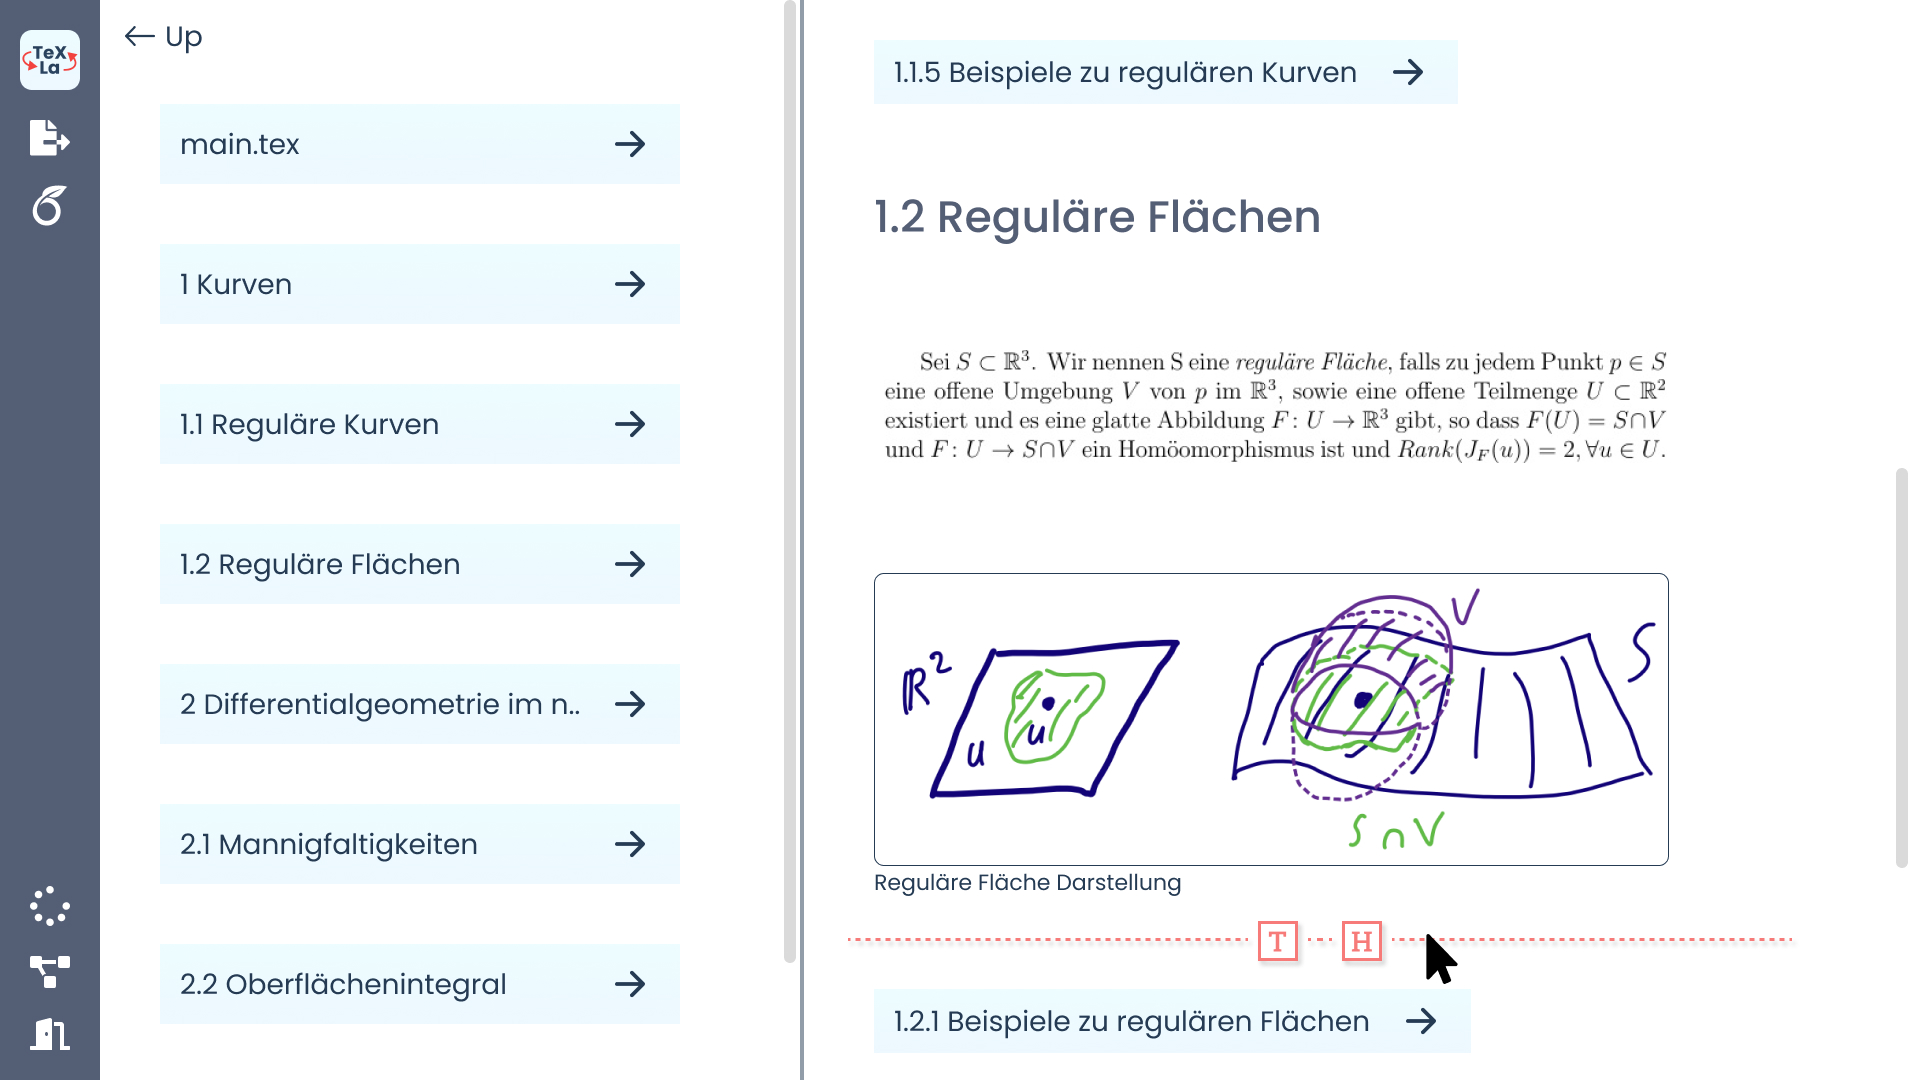
\includegraphics[width=\textwidth]{assets/img/Item_Add_Hover}
  \captionof{figure}{Element hinzufügen durch Hovern}
\end{minipage}

Der User kann durch Hovern zwischen Elementen andere Elemente hinzufügen.
Der Zwischenraum, welcher mit dem neuen Element gefüllt werden soll, wird fokussiert.

\clearpage

\subsubsection{Abschnitt hinzufügen}

Nachdem der \enquote{Abschnitt hinzufügen}-Button gedrückt wurde, erscheint ein Popup-Fenster.

\begin{center}
  \begin{minipage}{0.5\linewidth}
    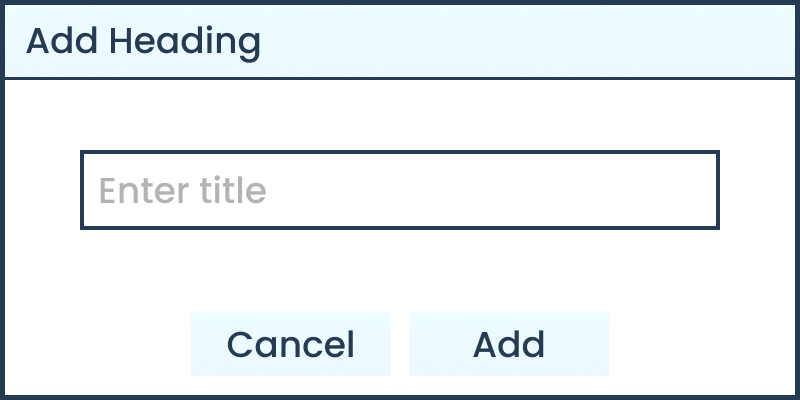
\includegraphics[width=\textwidth]{assets/img/Add_Heading_Box}
    \captionof{figure}{Abschnitt hinzufügen}
  \end{minipage}
\end{center}

Im \enquote{Abschnitt hinzufügen}-Fenster kann der User eine Überschrift für einen neuen Abschnitt eingeben und den
Vorgang bestätigen oder abbrechen.

\clearpage
\clearpage

\section{Qualitätszielbestimmungen}
\label{sec:qualitaetszielbestimmungen}

\subsection*{Performance}
\label{subsec:performance}

\nonFunctionality{Startdauer}{nfc:time-prog-start}

Die Anwendung benötigt maximal 10~\si{\second}, um zu starten,
also vom Absetzen des Befehls bis zum vollständig geladenen Frontend.

\nonFunctionality{Interaktionsdauer}{nfc:time-prog-restruct}

Das Verschieben, Erstellen und Löschen eines Elements benötigt jeweils maximal 0,5~\si{\second}.

\nonFunctionality{Export- und Speicherdauer}{nfc:time-save-export}

Das Exportieren oder Speichern von Dateien benötigt maximal 5~\si{\second}.

\nonFunctionality{Ressourcenverbrauch}{nfc:ressource-usage}

Die Anwendung benötigt maximal 4~\si{\giga\byte} Arbeitsspeicher.

\subsection*{Sicherheit}
\label{subsec:sicherheit}

\nonFunctionality{Verbindung zu Overleaf}{nfc:secure-connection}

Der Datenaustausch mit Overleaf erfolgt verschlüsselt über HTTPS.

\subsection*{Usability}
\label{subsec:usability}

\nonFunctionality{GUI-Design}{nfc:gui-design}

Die Anwendung wird in einem modernen Design umgesetzt.

\nonFunctionality{Bedienbarkeit}{nfc:ux-design}

Die Anwendung ist übersichtlich, intuitiv und einfach zu bedienen.

\subsection*{Wartbarkeit}
\label{subsec:wartbarkeit}

\nonFunctionality{Modularität}{nfc:modular-architecture}

Die Anwendung kann durch ihr modulares Design einfach um neue Module erweitert werden.
Bestehende Module können einfach modifiziert werden.

\clearpage
\clearpage

\section{Testfallszenarien}
\label{sec:testfallszenarien}

\subsection{Funktionale Testfälle}
\label{subsec:funktionale-testfaelle}

Die folgenden Testfälle testen die verpflichtenden funktionalen Anforderungen:

\test{Starten der Anwendung}{tst:start-01}
\begin{itemize}
  \item Vorbedingung: Dateistruktur erfüllt die Voraussetzungen (siehe~\ref{sec:produktleistungen}).
  \item Aktion: Programmstart durch Übergabe eines Dateipfades als Argument an die ausführbare Datei.
  \item Nachbedingung: Standardansicht in der höchsten Ebene der Anwendung.
\end{itemize}
\tests{fnc:start}

\test{Beenden der Anwendung}{tst:stop-01}
\tests{fnc:exit}
\begin{itemize}
  \item Vorbedingung: Die Anwendung ist aktiv und befindet sich in irgendeinem Ansichtsmodus.
  \item Aktion: Klicken des Exit-Symbols in der unteren linken Ecke der Sidebar.
  \item Nachbedingung: Die Anwendung wird geschlossen.
  Die lokalen und Remote-Repositories sind synchron mit den vom Benutzer in \texla{} vorgenommenen Änderungen.
\end{itemize}

\test{Hierarchische Darstellung}{tst:hierarchy-01}
\tests{fnc:hierarchy}
\begin{itemize}
  \item Vorbedingung: Das \texla"=Pflichtenheft ist lokal verfügbar.
  \item Aktion: Öffnen der \texla"=Anwendung mit dem Dateipfad zum \texla"=Pflichtenheft.
  \item Nachbedingung: Alle unterstützten Strukturelemente wurden erkannt und korrekt dargestellt.
\end{itemize}

\clearpage

\test{Unterstützung inkludierter Dateien}{tst:input-01}
\tests{fnc:input}
\begin{itemize}
  \item Vorbedingung: \LaTeX"=Datei mit \verb|/input| steht lokal zur Verfügung.
  \texla{} ist gestartet.
  \item Aktion: Navigation zum Strukturelement des \verb|/input|-Makros.
  \item Nachbedingung: Die Datei wurde erkannt und wird angezeigt.
\end{itemize}

\test{Strukturelemente in Blöcke aufteilen}{tst:blocks-01}
\tests{fnc:blocks}
\begin{itemize}
  \item Vorbedingung: \LaTeX"=Datei enthält \verb|/begin{...} ... /end{...}|.
  \texla{} ist gestartet.
  \item Aktion: Navigation zur definierten Umgebung.
  \item Nachbedingung: Das Umgebungs-Strukturelement wurde erkannt und korrekt angezeigt.
\end{itemize}

\test{Rendering von Bildern}{tst:render-01}
\tests{fnc:render}
\begin{itemize}
  \item Vorbedingung: \LaTeX"=Datei mit \verb|/includegraphics| steht lokal zur Verfügung.
  \texla{} ist gestartet.
  \item Aktion: Navigation zum definierten Bild.
  \item Nachbedingung: Das Bild-Strukturelement wurde erkannt und korrekt gerendert.
\end{itemize}

\test{Rendering von mathematischen Formeln}{tst:render-02}
\tests{fnc:render}
\begin{itemize}
  \item Vorbedingung: \LaTeX"=Datei mit \verb|/begin{displaymath} ... /end{displaymath}| steht lokal zur Verfügung.
  \texla{} ist gestartet.
  \item Aktion: Navigation zur definierten Formel.
  \item Nachbedingung: Die mathematische Formel wurde erkannt und korrekt gerendert.
\end{itemize}

\clearpage

\test{Formatierung in Textblöcken}{tst:format-01}
\tests{fnc:format}
\begin{itemize}
  \item Vorbedingung: \LaTeX"=Datei mit \verb|/textbf| und \verb|/textit| steht lokal zur Verfügung.
  \texla{} ist gestartet.
  \item Aktion: Navigation zum enthaltenden Strukturelement.
  \item Nachbedingung: Fetter und kursiver Text wurde gerendert.
\end{itemize}

\test{Ein- und Ausblenden sowie Komprimieren von Strukturelementen}{tst:clarity-01}
\tests{fnc:hide}
\tests{fnc:compact}
\begin{itemize}
  \item Vorbedingung: \LaTeX"=Datei mit mehrstufiger Gliederung (\zB{} \verb|/section| und \verb|/subsection|) steht
  lokal zur Verfügung.
  \texla{} ist gestartet.
  \item Aktion: Navigation zum Strukturelement.
  Ein Strukturelement wird in der Strukturspalte angeklickt.
  \item Nachbedingung: Die Überschriften der Strukturelemente werden kompakt in der Strukturspalte angezeigt.
  Verborgene und erweiterbare Elemente werden kompakt in der Lesespalte angezeigt.
\end{itemize}

\test{Erkennen von Algorithmen}{tst:compact-02}
\tests{fnc:compact}
\begin{itemize}
  \item Vorbedingung: \LaTeX"=Datei mit Algorithmus-Umgebung steht lokal zur Verfügung.
  \texla{} ist gestartet.
  \item Aktion: Navigation zur Ebene oberhalb des definierten Algorithmus.
  \item Nachbedingung: Das Algorithmus-Strukturelement wird in Kompaktform durch den Text \enquote{Algorithmus} bzw.
  \enquote{algorithm} repräsentiert.
\end{itemize}

\test{Bereitstellung einer Graphansicht}{tst:graph-01}
\tests{fnc:graph}
\begin{itemize}
  \item Vorbedingung: \texla{} ist gestartet auf validem \LaTeX"=Dokument.
  \item Aktion: Klicken auf den Ansichtwechsel-Button.
  \item Nachbedingung: Die Graphansicht wird angezeigt.
\end{itemize}

\test{Legale Verschiebung von Elementen per Drag and Drop}{tst:dragdrop-01}
\tests{fnc:drag-and-drop}
\begin{itemize}
  \item Vorbedingung: \texla{} ist gestartet auf validem \LaTeX"=Dokument.
  \item Aktion: Navigation zum Strukturelement.
  In der Lesespalte wird ein Element angeklickt und nach oben oder unten, vor oder nach ein anderes Element
  verschoben.
  \item Nachbedingung: Das Element steht an der gewünschten Position.
\end{itemize}

\test{Illegale Verschiebung von Elementen per Drag and Drop}{tst:dragdrop-02}
\tests{fnc:drag-and-drop}
\begin{itemize}
  \item Vorbedingung: \LaTeX"=Datei mit mehrstufiger Gliederung (\zB{} \verb|/section| und \verb|/subsection|) steht
  lokal zur Verfügung.
  \texla{} ist gestartet.
  \item Aktion: Navigation zum Strukturelement.
  In der Lesespalte wird ein Element angeklickt und zur Strukturspalte verschoben.
  \item Nachbedingung: Das Element behält seine ursprüngliche Position.
\end{itemize}

\test{Bereitstellung eines Minieditors}{tst:minieditor-01}
\tests{fnc:minieditor}
\begin{itemize}
  \item Vorbedingung: \texla{} ist gestartet auf validem \LaTeX"=Dokument mit mindestens einem textuellen Absatz.
  \item Aktion: Navigation zum und Anklicken eines textuellen Absatzes im Arbeitsbereich.
  Anklicken des Absatzes in der Lesespalte.
  Navigation zum Kontextmenü und Anklicken des Bearbeitungsmodus.
  \item Nachbedingung: Die linke Spalte wird schmaler angezeigt.
  Der Minieditor für den ausgewählten Absatz wird auf der rechten Seite angezeigt.
\end{itemize}

\clearpage

\test{Hinzufügen von Abschnitten}{tst:add-01}
\tests{fnc:add}
\begin{itemize}
  \item Vorbedingung: \texla{} ist gestartet auf validem \LaTeX"=Dokument.
  \item Aktion: Navigation zur Lesespalte.
  In der Standardansicht hinter oder zwischen beliebigen Elementen hovern.
  Klicken des H-Button, wodurch ein Popup erscheint.
  Hinzufügen einer Überschrift.
  \item Nachbedingung: Das neue Element wird in der Standardansicht angezeigt.
\end{itemize}

\test{Hinzufügen von \LaTeX"=Blöcken}{tst:add-02}
\tests{fnc:add}
\begin{itemize}
  \item Vorbedingung: \texla{} ist gestartet auf validem \LaTeX"=Dokument.
  \item Aktion: Navigation zur Lesespalte.
  In der Standardansicht hinter oder zwischen beliebigen Elementen hovern.
  Klicken des T-Button, wodurch \texla{} in den Bearbeitungsmodus wechselt.
  Bearbeitung und Speichern.
  \item Nachbedingung: Der neue \LaTeX"=Block wird in der Standardansicht angezeigt.
\end{itemize}

\test{Verschmelzen von zwei Textabsätzen}{tst:add-03}
\tests{fnc:add}
\begin{itemize}
  \item Vorbedingung: \LaTeX"=Datei mit mindestens zwei textuellen Absätzen auf gleicher Ebene steht lokal zur
  Verfügung.
  \texla{} ist gestartet.
  \item Aktion: Navigation zur Lesespalte.
  Bearbeiten im Minieditor des unteren von zwei textuellen Absätzen.
  Klicken der Rücktaste am Anfang des Absatzes.
  \item Nachbedingung: Die beiden Strukturelemente wurden verschmolzen.
\end{itemize}

\clearpage

\test{Benutzerdefinierter Export}{tst:export-01}
\tests{fnc:export}
\begin{itemize}
  \item Vorbedingung: \texla{} ist gestartet auf validem \LaTeX"=Dokument.
  \item Aktion: Navigation zur Sidebar und Auswahl der Export-Option.
  Auswahl von Exportmöglichkeiten in einem Pop-up-Fenster der GUI.
  \item Nachbedingung: Die exportierte Datei steht mit den ausgewählten Optionen zur Verfügung.
\end{itemize}

\test{Integration mit Git}{tst:git-01}
\tests{fnc:git}
\begin{itemize}
  \item Vorbedingung: \texla{} ist gestartet.
  \item Aktion: Verändern der \LaTeX"=Datei mit \texla{}.
  Abwarten von 5~\si{\second}.
  \item Nachbedingung: Ein Commit wurde im lokalen Repository durchgeführt.
  Ein Push wurde zum Remote-Repository durchgeführt.
\end{itemize}

\test{Link zum Projekt in Overleaf}{tst:overleaf-01}
\tests{fnc:overleaf-link}
\begin{itemize}
  \item Vorbedingung: \texla{} ist gestartet auf validem \LaTeX"=Dokument.
  \item Aktion: Navigation zur Sidebar und Auswahl der Overleaf-Option.
  \item Nachbedingung: Der Browser öffnet sich mit dem Projekt in Overleaf.
\end{itemize}

Die folgenden Testfälle testen die optionalen funktionalen Anforderungen:

\test{Konfigurierbare graphische Oberfläche}{tst:gui-01}
\tests{fnc:configurable-gui}
\begin{itemize}
  \item Vorbedingung: \texla{} ist gestartet auf validem \LaTeX"=Dokument mit \LaTeX"=Kommentaren.
  \item Aktion: Navigation zur Sidebar und Auswahl der Option \enquote{Ausblenden von \LaTeX"=Kommentaren}.
  \item Nachbedingung: \LaTeX"=Kommentare werden nicht mehr angezeigt.
\end{itemize}

\test{Tastaturkürzel für häufige Operationen}{tst:keyboard}
\tests{fnc:keyboard}
\begin{itemize}
  \item Vorbedingung: \texla{} ist gestartet auf validem \LaTeX"=Dokument.
  \item Aktion: Drücken der Tastenkombination zum Wechseln zwischen Modi.
  \item Nachbedingung: \texla{} wechselt zwischen Standard- und Graphmodus.
\end{itemize}

\test{Hinzufügen von Notizen}{tst:notes-01}
\tests{fnc:notes}
\tests{fnc:meta-comments}
\begin{itemize}
  \item Vorbedingung: \LaTeX"=Datei mit mindestens einem Strukturelement steht lokal zur Verfügung.
  \texla{} ist gestartet.
  \item Aktion: Navigation zum Strukturelement.
  Öffnen des Kontextmenüs zu einem Strukturelement.
  Auswahl der Notiz-Option und Bearbeitung in einem Pop-up-Fenster der GUI.
  \item Nachbedingung: Die Notiz wird als Meta-Kommentar im Quelltext gespeichert.
\end{itemize}

\test{Benutzerdefinierte Kompaktformen von Strukturelementen}{tst:compact-01}
\tests{fnc:manual-compact-form}
\begin{itemize}
  \item Vorbedingung: \LaTeX"=Datei mit mindestens einem Strukturelement steht lokal zur Verfügung.
  \texla{} ist gestartet.
  \item Aktion: Navigation zum Strukturelement.
  Öffnen des Kontextmenüs zu einem Strukturelement.
  Auswahl der Kompaktform-Option und Eingeben einer Zusammenfassung.
  \item Nachbedingung: Das Strukturelement wird an den entsprechenden Stellen in der neuen Kompaktform angezeigt.
\end{itemize}

\clearpage

\test{Syntax-Hervorhebung im Texteditor}{tst:syntax-highlighting-01}
\tests{fnc:syntax-highlighting}
\begin{itemize}
  \item Vorbedingung: \LaTeX"=Datei mit mindestens einem Strukturelement steht lokal zur Verfügung.
  \texla{} ist gestartet.
  \item Aktion: Navigation zum Strukturelement.
  Öffnen des Kontextmenüs zu diesem Strukturelement.
  Auswahl der Bearbeiten-Option.
  \item Nachbedingung: Die \LaTeX"=Befehle des Strukturelements werden im Minieditor farblich hervorgehoben.
\end{itemize}

\test{Code-Vervollständigung im Texteditor}{tst:gcode-completion}
\tests{fnc:code-completion}
\begin{itemize}
  \item Vorbedingung: \LaTeX"=Datei mit mindestens einem textuellen Strukturelement steht lokal zur Verfügung.
  \texla{} ist gestartet.
  \item Aktion: Navigation zum Strukturelement.
  Öffnen des Kontextmenüs zu diesem Strukturelement.
  Wechsel in den Bearbeitungsmodus.
  Eingabe von \LaTeX"=Befehlen.
  \item Nachbedingung: \LaTeX"=Befehle werden automatisch vervollständigt.
\end{itemize}

\test{Möglichkeit zur einfachen Übersetzung der Anwendung}{tst:multilingual}
\tests{fnc:multilingual}
\begin{itemize}
  \item Vorbedingung: \texla{} ist gestartet.
  \item Aktion: Navigation zur Sidebar, Anklicken der Option \enquote{Sprache} und Auswahl einer bestimmten Sprache.
  \item Nachbedingung: Die Sprache der Anwendung wurde zur ausgewählten Sprache geändert.
\end{itemize}

\clearpage

\test{Kompatibilität mit Browser-Extensions zur Autokorrektur}{tst:autocorrect}
\tests{fnc:autocorrect}
\begin{itemize}
  \item Vorbedingung: \texla{} ist gestartet.
  Die Browser-Extension LanguageTool ist installiert und aktiv.
  \item Aktion: Im Bearbeitungsmodus wird Text eingegeben, der bezüglich Grammatik oder Rechtschreibung fehlerhaft
  ist.
  \item Nachbedingung: Fehlerhafte Teile des Textes werden erkannt und entsprechend hervorgehoben.
\end{itemize}

\test{Automatische Zusammenfassung von Abschnitten durch KI}{tst:ai-tldrs}
\tests{fnc:ai-tldrs}
\begin{itemize}
  \item Vorbedingung: \texla{} ist gestartet auf validem \LaTeX"=Dokument.
  \item Aktion: Navigation zur Sidebar und Auswahl der Option \enquote{KI-Zusammenfassung}.
  \item Nachbedingung: Die einzelnen Zusammenfassungen pro Abschnitt wurden automatisch generiert.
\end{itemize}

\test{Unterstützung beim Schreiben durch KI}{tst:ai-rewriting}
\tests{fnc:ai-rewriting}
\begin{itemize}
  \item Vorbedingung: \texla{} ist gestartet auf validem \LaTeX"=Dokument.
  \item Aktion: Navigation zur Sidebar und Auswahl eines Strukturelements.
  Wechsel in den Bearbeitungsmodus.
  Eingabe einer Anfrage an die KI.
  \item Nachbedingung: Die KI hat eine Antwort zur Anfrage geschrieben.
\end{itemize}

\test{Bereitstellung als reinen Online-Dienst}{tst:online}
\tests{fnc:online}
\begin{itemize}
  \item Vorbedingung: Internetverbindung ist vorhanden.
  \item Aktion: \texla{} wird im Browser geöffnet.
  \item Nachbedingung: Dokumente können mit \texla{} online bearbeitet werden.
\end{itemize}

\clearpage

\test{Voreinstellungsprofile für den benutzerdefinierten Export}{tst:export-profiles}
\tests{fnc:export-profiles}
\begin{itemize}
  \item Vorbedingung: \texla{} ist gestartet.
  \item Aktion: Navigation zur Sidebar.
  Anklicken der Option \enquote{Export} und Auswahl eines voreingestellten Profils.
  \item Nachbedingung: Die Export-Einstellungen wurden entsprechend des Profils geändert.
\end{itemize}

\test{Export von PDF-Dateien}{tst:pdf-export}
\tests{fnc:pdf-export}
\begin{itemize}
  \item Vorbedingung: \texla{} ist gestartet auf validem \LaTeX"=Dokument.
  \item Aktion: Navigation zur Sidebar und Auswahl der Export-Option.
  \item Nachbedingung: Das \LaTeX"=Dokument wurde als PDF exportiert.
\end{itemize}

\test{Verschieben von Listenelementen per Drag and Drop}{tst:list-dnd}
\tests{fnc:lists}
\begin{itemize}
  \item Vorbedingung: \texla{} ist gestartet auf validem \LaTeX"=Dokument mit einer \verb|itemize|-Umgebung mit
  mindestens zwei Elementen.
  \item Aktion: Navigation zur Liste.
  Verschieben eines Listeneintrags per Drag and Drop.
  \item Nachbedingung: Listeneinträge erscheinen in neuer Reihenfolge.
\end{itemize}

\subsection{Szenarien}
\label{subsec:tests-scenarios}

Anmerkung: Jegliche Ähnlichkeit zu real existierenden Personen ist rein zufällig.

\subsubsection{Erweiterung und Verwaltung eines bestehenden \LaTeX"=Projekts}

Der Benutzer Paul hat das Ziel, sein umfangreiches \LaTeX"=Projekt zu erweitern und zu verwalten.
Bedauerlicherweise hat er aufgrund der Vielzahl an Dateien den Überblick verloren und einige \LaTeX"=Befehle sind
ihm entfallen, was sein Verständnis der einzelnen Abschnitte erschwert.

Paul navigiert zum lokalen Dateipfad seines Projekts und startet die \texla"=Anwendung mit einem Konsolenbefehl.
Nun befindet er sich in der Hauptansicht der Anwendung in seinem Browser und erblickt auf der linken
Seite die Sidebar.

Zunächst möchte Paul einen Gesamtüberblick über das Projekt gewinnen.
Hierzu wechselt er über die Sidebar in den Graphmodus und betrachtet die Baumansicht aller Elemente.
Dabei bemerkt er, dass ein Abschnitt zu groß geworden ist, weshalb er einen Unterabschnitt zu einem separaten Abschnitt
umwandeln will.
Mithilfe der Drag-and-Drop-Funktion passt er die Anordnung des Unterabschnitts an und wechselt dann zurück in den
Standardmodus.

Paul sieht nun auf der linken Seite eine kompakte Strukturspalte
mit Überschriften, die den verschiedenen Abschnitten zugeordnet sind.
Nun möchte er einen bestimmten Abschnitt bearbeiten und klickt hierzu auf die entsprechende kompakte Überschrift.
In der Lesespalte auf der rechten Seite werden ihm nun alle Elemente angezeigt, die zu diesem Abschnitt
gehören, sowie alle projizierten Elemente aus vorhergehenden Ebenen.
Er wählt ein Textelement und klickt den Bearbeitungsbutton.
Im Bearbeitungsmodus führt er die gewünschten Änderungen durch und speichert diese.

Im Anschluss stellt Paul fest, dass die Reihenfolge der Elemente optimiert werden könnte.
Er nutzt erneut die Drag-and-Drop-Funktion, um eine Überschrift hinter eine andere zu verschieben.

Zufrieden mit seinen Anpassungen schließt Paul die Anwendung.
All seine Änderungen wurden sowohl lokal als auch remote gespeichert.

\subsubsection{Unterstützung bei der Strukturverbesserung eines \LaTeX"=Projekts}

Benutzer Max verfolgt das Ziel, seinem Kommilitonen Paul bei der Verbesserung der Struktur seines
\LaTeX"=Projekts zu unterstützen.
Dafür setzt er die \texla"=Anwendung ein, um Paul hilfreiche Notizen zu hinterlassen.

Max betrachtet zunächst die Überschriften in der Strukturspalte und durchläuft diese systematisch.
Dabei bemerkt er, dass einige Abschnitte stilistisch inkorrekt formatiert sind.
Da es Max ein Anliegen ist, dass Paul einen korrekten \LaTeX"=Stil erlernt, entscheidet
er sich dagegen, das Problem eigenhändig zu beheben.

Stattdessen wählt er die Überschrift des betroffenen Elements und navigiert zur Lesespalte.
Er bewegt den Cursor über einen Abschnitt und wählt die Option des Minieditors.
Hier hinterlässt er für Paul wichtige Bearbeitungshinweise in Form von \LaTeX"=Kommentaren.

Schließlich beendet Max die Anwendung und teilt Paul die hinterlassenen Bearbeitungshinweise mit.

\subsubsection{Verbesserung von Algorithmen-Vorlesungsfolien}

Benutzer Linus, der an einer Universität als Tutor tätig ist, strebt danach, die \LaTeX"=Folien für die
Algorithmen-Vorlesung zu verbessern.
Sein Lehrstuhl bevorzugt die Nutzung von Overleaf, auf welchem auch die aktuellen Folien abgelegt sind.
Linus erkennt Optimierungspotenzial bei einigen Pseudocode-Algorithmen.
Allerdings sind die vorhandenen Pseudocode-Algorithmen aufgrund des unorganisierten \LaTeX"=Repositorys schwer
auffindbar.

Daher entscheidet er sich für den Einsatz von \texla{}.
Linus wechselt in den Graphmodus und erhält einen Überblick
über verschiedene Algorithmen-Blöcke in Form eines Baumes.
Durch die Auswahl eines Algorithmus-Blocks wechselt er in den
Standardmodus, und der ausgewählte Algorithmus ist nun in der Lesespalte auf der rechten Seite zu finden.
Mithilfe des Bearbeitungsmodus und des Minieditors optimiert er diese Blöcke.

Während der Bearbeitung kommt ihm eine brillante Idee.
Linus erstellt ein neues Element zwischen zwei bestehenden Abschnitten und bringt seine Idee dort unter.
Er möchte noch ein Bild zur Illustration beifügen, das er in den Ordner der \LaTeX"=Datei legt und noch in demselben
Minieditor einbindet.
Nach der Bestätigung im Minieditor werden der neue Absatz und das Bild als zwei getrennte Strukturelemente angezeigt.

Nach Abschluss der Bearbeitung möchte er seine Idee mit einem externen Freund von der Universität teilen.
Er stellt jedoch fest, dass er nicht die Berechtigung hat, ihn zum Repository des Lehrstuhls einzuladen.
Daher entscheidet er sich, das \LaTeX"=Dokument zu exportieren.
In den Exporteinstellungen wählt Linus aus, dass alles exportiert werden soll.
Schließlich sendet er die Datei an seinen Freund.

\clearpage
\clearpage

\section{Entwicklungsumgebung}
\label{sec:entwicklungsumgebung}

Zur Entwicklung der Anwendung werden verschiedene IDEs von JetBrains wie IntelliJ IDEA, WebStorm und CLion verwendet.
Zur Versionsverwaltung und zur allgemeinen Projektverwaltung wird Git in Verbindung mit GitLab verwendet.

\clearpage
\clearpage

\section{Glossar}
\label{sec:glossar}

% für Begriffe, die bei uns besondere Bedeutung haben
\setlength{\extrarowheight}{2em}

\begin{longtable}{>{\bfseries}rp{9cm}}
  Absatz &
  Ein durch Leerzeilen abgetrenntes Stück Text. \\

  Abschnitt &
  Gibt Elementen einen semantischen Rahmen.
  Entspricht in \LaTeX{} \verb|part|, \verb|chapter|, \verb|section|, \verb|subsection|, \verb|subsubsection|,
  \verb|paragraph| oder \verb|subparagraph|. \\

  Arbeitsbereich &
  Bereich rechts von der Sidebar, welcher zur Restrukturierung genutzt wird.
  Der Bereich kann zwischen dem Standardmodus, dem Graphmodus und dem Bearbeitungsmodus wechseln. \\

  AST &
  Abstract Syntax Tree, abstrakter Syntaxbaum.
  Eine Datenstruktur, die typischerweise zum Speichern von und Arbeiten auf strukturell verschachtelten Dokumenten
  verwendet wird. \\

  CLI &
  Command Line Interface, Befehlszeilenschnittstelle. \\

  Element, Strukturelement &
  Das Dokument wird in Elemente gegliedert, wie zum Beispiel Abschnitte, Bilder oder \LaTeX"=Blöcke.
  Elemente sind restrukturierbar und können weitere Elemente als Kinder enthalten. \\

  Expandable &
  Element mit ausklappbarem Inhalt, also ein Abschnitt oder Input. \\

  GUI, Frontend &
  Graphical User Interface, grafische Benutzeroberfläche.
  Im Browser sichtbarer Teil der Applikation. \\

  Inline-Makro &
  Ein Makro, das innerhalb eines Textabsatzes vorkommt.
  Es wird als Quelltext angezeigt, also semantisch ignoriert. \\

  Input &
  Ein Element basierend auf einer mit \verb|input| eingebundenen \LaTeX"=Datei. \\

  Kommentar &
  Vom User geschriebener Kommentar im Quelltext. \\

  Kompaktform &
  Eine Kurzzusammenfassung eines Elements, also zum Beispiel die Überschrift eines Abschnitts, der Name einer
  inkludierten Datei oder die ersten Worte eines Absatzes. \\

  \LaTeX"=Block &
  Ein Element, das einen nicht zu parsenden Teil des Dokuments darstellt, wie zum Beispiel Makros oder nicht
  unterstützte Umgebungen. \\

  Minieditor &
  Der Texteditor in der GUI, der es erlaubt, \LaTeX"=Quelltext von Strukturelementen zu bearbeiten. \\

  Notiz &
  Freitext-Zusatzinformation zu einem Strukturelement, meistens nicht sichtbar. \\

  REST-API &
  Representational State Transfer Application Programming Interface.
  Zustandslose Computerschnittstelle für die Kommunikation zwischen Frontend und Backend. \\

  Überschrift &
  Die Überschrift eines Abschnitts. \\

  Zusatzinformation, Attribut &
  An einem Strukturelement gespeicherte zusätzliche Informationen, die nicht zum \LaTeX"=Quelltext selbst gehören,
  zum Beispiel Notizen. \\
\end{longtable}


% inputs in verbatim environments are manipulated, so sections 5, 8, 11 and 13 are slightly modified

\end{document}
